\section{Структура разделов и описание страниц}
\subsection{Структура разделов}
Все названия разрабатываемых страниц и разделов сайта являются условными и могут корректироваться по согласованию с Заказчиком в ходе проектирования.

Ниже представлена первоначальная структура разделов «Учебные материалы», «Генератор вариантов», а также административной панели управления данными разделами.

\subsubsection{Раздел «Учебные материалы»}
\begin{itemize}
	\item ЕГЭ профильного уровня
	\begin{itemize}
		\item Содержание
		\begin{itemize}
			\item Задания
		\end{itemize}
	\end{itemize}

	\item ЕГЭ базового уровня
	\begin{itemize}
		\item Содержание
		\begin{itemize}
			\item Задания
		\end{itemize}
	\end{itemize}

	\item ОГЭ
	\begin{itemize}
		\item Содержание
		\begin{itemize}
			\item Задания
		\end{itemize}
	\end{itemize}

	\item Высшая математика
	\begin{itemize}
		\item Содержание
		\begin{itemize}
			\item Задания
		\end{itemize}
	\end{itemize}

	\item Учебные пособия
	\begin{itemize}
		\item Список учебных пособий
	\end{itemize}

	\item Презентации
	\begin{itemize}
		\item Список презентаций
	\end{itemize}

	\item Авторизация в административной панели
\end{itemize}

\subsubsection{Раздел «Генератор вариантов»}
\begin{enumerate}
	\item Генератор вариантов
	\begin{enumerate}
		\item Тестовый вариант
		\begin{enumerate}
			\item Версия для печати
			\item Версия для скачивания
		\end{enumerate}
	\end{enumerate}
\end{enumerate}

\subsubsection{Административная панель}
\begin{itemize}
	\item Административная панель. Главная страница

	\item Список задач
	\begin{itemize}
		\item Создать/редактировать задачу
		\item Импортировать задачу
	\end{itemize}

	\item Список разделов
	\begin{itemize}
		\item Создать/редактировать раздел
	\end{itemize}

	\item Список пособий
	\begin{itemize}
		\item Добавить/редактировать пособие
	\end{itemize}

	\item Список презентаций
	\begin{itemize}
		\item Добавить/редактировать презентацию
	\end{itemize}
\end{itemize}

Карта разрабатываемых разделов приведена в приложении 1 данного технического задания.

\subsection{Описание страниц. Административная часть}
\subsubsection{Страница «Главная»}
\begin{figure}[H]
	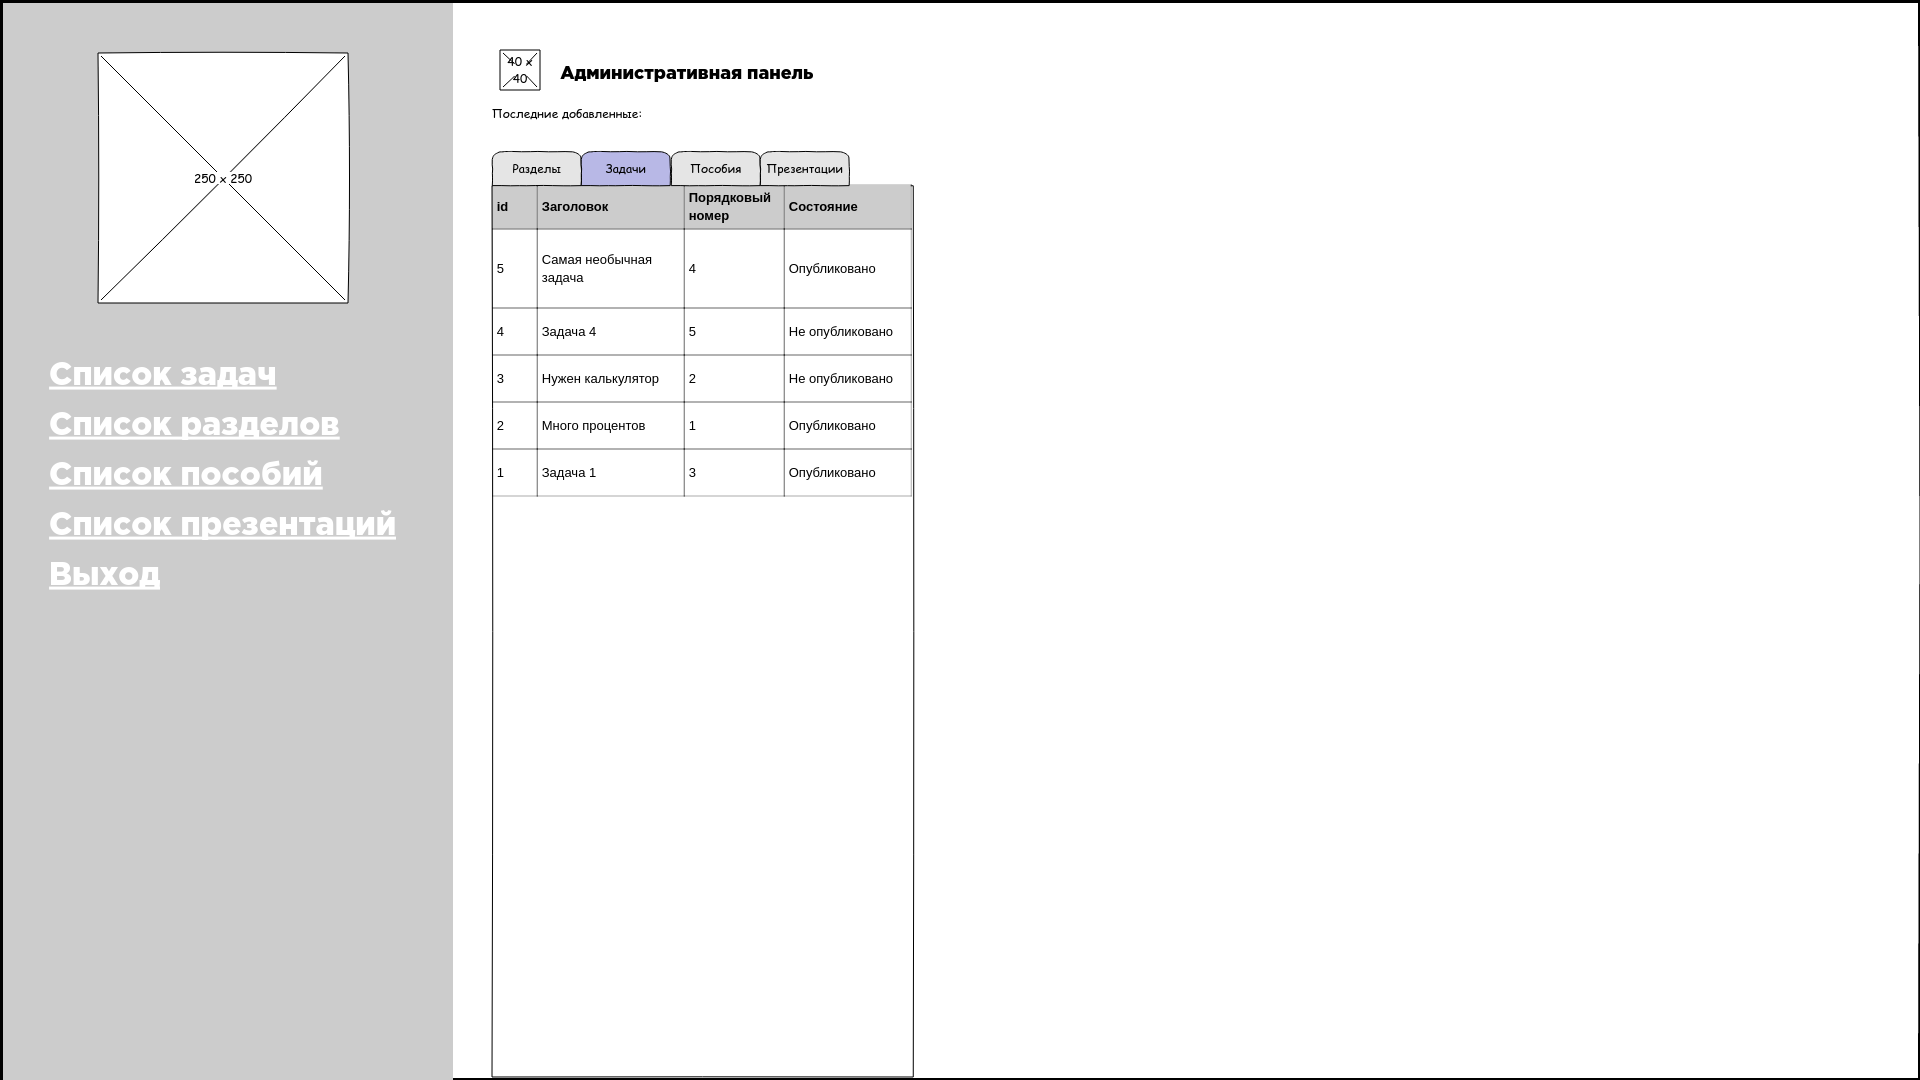
\includegraphics[width=\textwidth]{5-2-1}
\end{figure}
\paragraph{Назначение страницы:}
Главная страница предназначена для навигации в административной панели.

\paragraph{Структура страницы}
\begin{enumerate}
	\item Шапка
	\begin{enumerate}
		\item Заголовок
	\end{enumerate}

	\item Меню
	\begin{enumerate}
		\item  Логотип
		\item  Навигация
	\end{enumerate}

	\item  Контент
	\begin{enumerate}
		\item  Таблица последних действий
	\end{enumerate}
\end{enumerate}

\paragraph{Функциональные возможности}
\begin{enumerate}
	\item Меню
	\begin{enumerate}
		\item Навигация
		\begin{enumerate}
			\item Переход между разделами
		\end{enumerate}
	\end{enumerate}

	\item Контент
	\begin{enumerate}
		\item Таблица последних действий
		\begin{enumerate}
			\item Просмотр последних действий во всех разделах .В основной части главной страницы расположена таблица с вкладками, отображающими краткую статистику по последним добавленным элементам:
			\begin{enumerate}
				\item  в списках разделов
				\item  в списках задач
				\item  в списках пособий
				\item  в списках презентаций
			\end{enumerate}
		\end{enumerate}
	\end{enumerate}
\end{enumerate}

\subsubsection{Страница «Список разделов»}
\begin{figure}[H]
	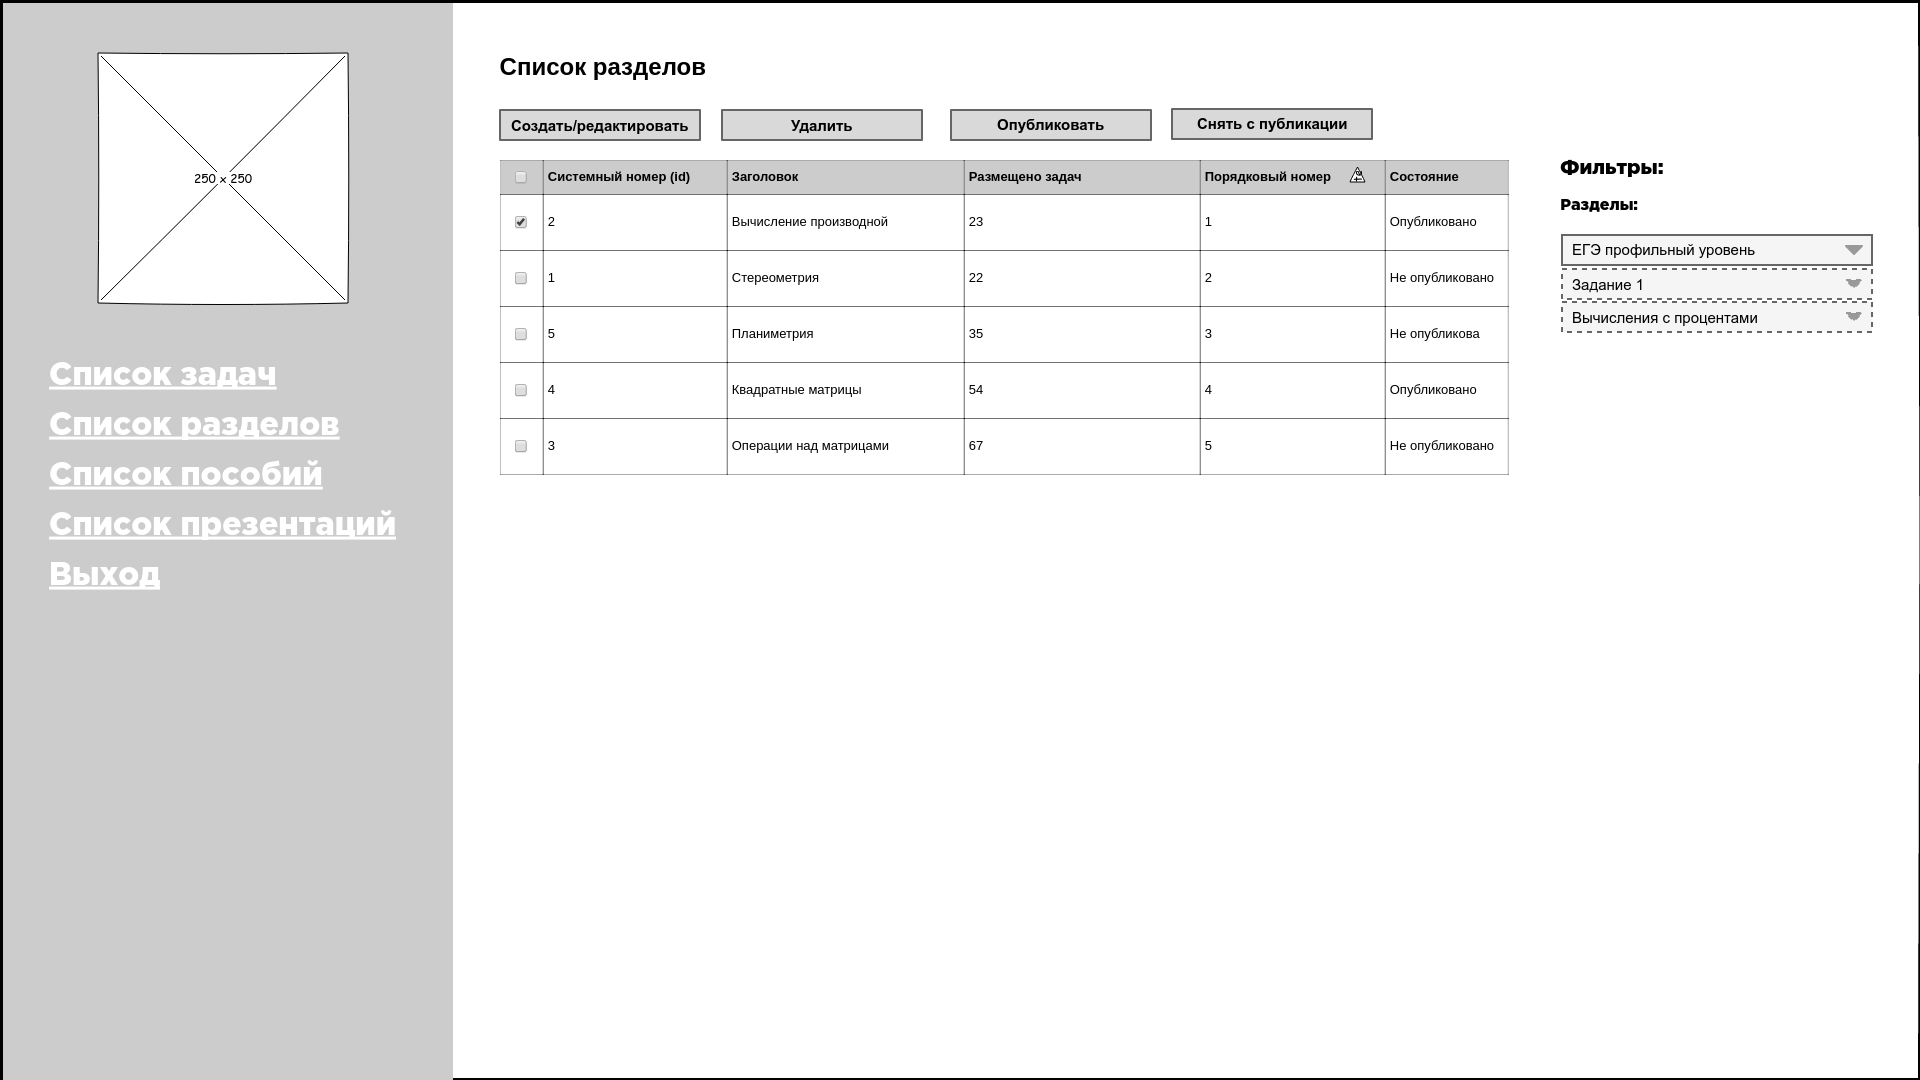
\includegraphics[width=\textwidth]{5-2-2}
\end{figure}
\paragraph{Назначение страницы:} предназначена для управления разделами всех уровней вложенности из категорий «ЕГЭ профильный уровень», «ЕГЭ базовый уровень», «ОГЭ», «Высшая математика».

\paragraph{Структура страницы}
\begin{enumerate}
	\item Шапка
	\begin{enumerate}
		\item Заголовок
	\end{enumerate}

	\item Меню
	\begin{enumerate}
		\item Логотип
		\item Навигация
	\end{enumerate}

	\item Сайдбар
	\begin{enumerate}
		\item Фильтры
		\begin{enumerate}
			\item Разделы
		\end{enumerate}
	\end{enumerate}

	\item Контент
	\begin{enumerate}
		\item Кнопки управления
		\begin{itemize}
			\item Создать/редактировать
			\item Удалить
			\item Опубликовать
			\item Снять с публикации
		\end{itemize}
		\item Таблица разделов
	\end{enumerate}
\end{enumerate}

\paragraph{Функциональные возможности}
\begin{enumerate}
	\item Меню
	\begin{enumerate}
		\item Навигация
		\begin{itemize}
			\item Переход между разделами
		\end{itemize}
	\end{enumerate}

	\item Сайдбар
	\begin{enumerate}
		\item Фильтры
		\begin{itemize}
			\item «Фильтрация» разделов
		\end{itemize}
	\end{enumerate}

	\item Контент
	\begin{enumerate}
		\item Таблица разделов
		\begin{itemize}
			\item Сортировка списка разделов по столбцам
		\end{itemize}

		\item Кнопки управления
		\begin{itemize}
			\item Создание раздела
			\item Редактирование раздела
			\item Удаление раздела или нескольких разделов
			\item Изменение состояния раздела на «Опубликовать»
			\item Изменение состояния раздела на «Снять с публикации»
		\end{itemize}
	\end{enumerate}
\end{enumerate}

\subsubsection{Страница «Создать/редактировать раздел»}
\begin{figure}[H]
	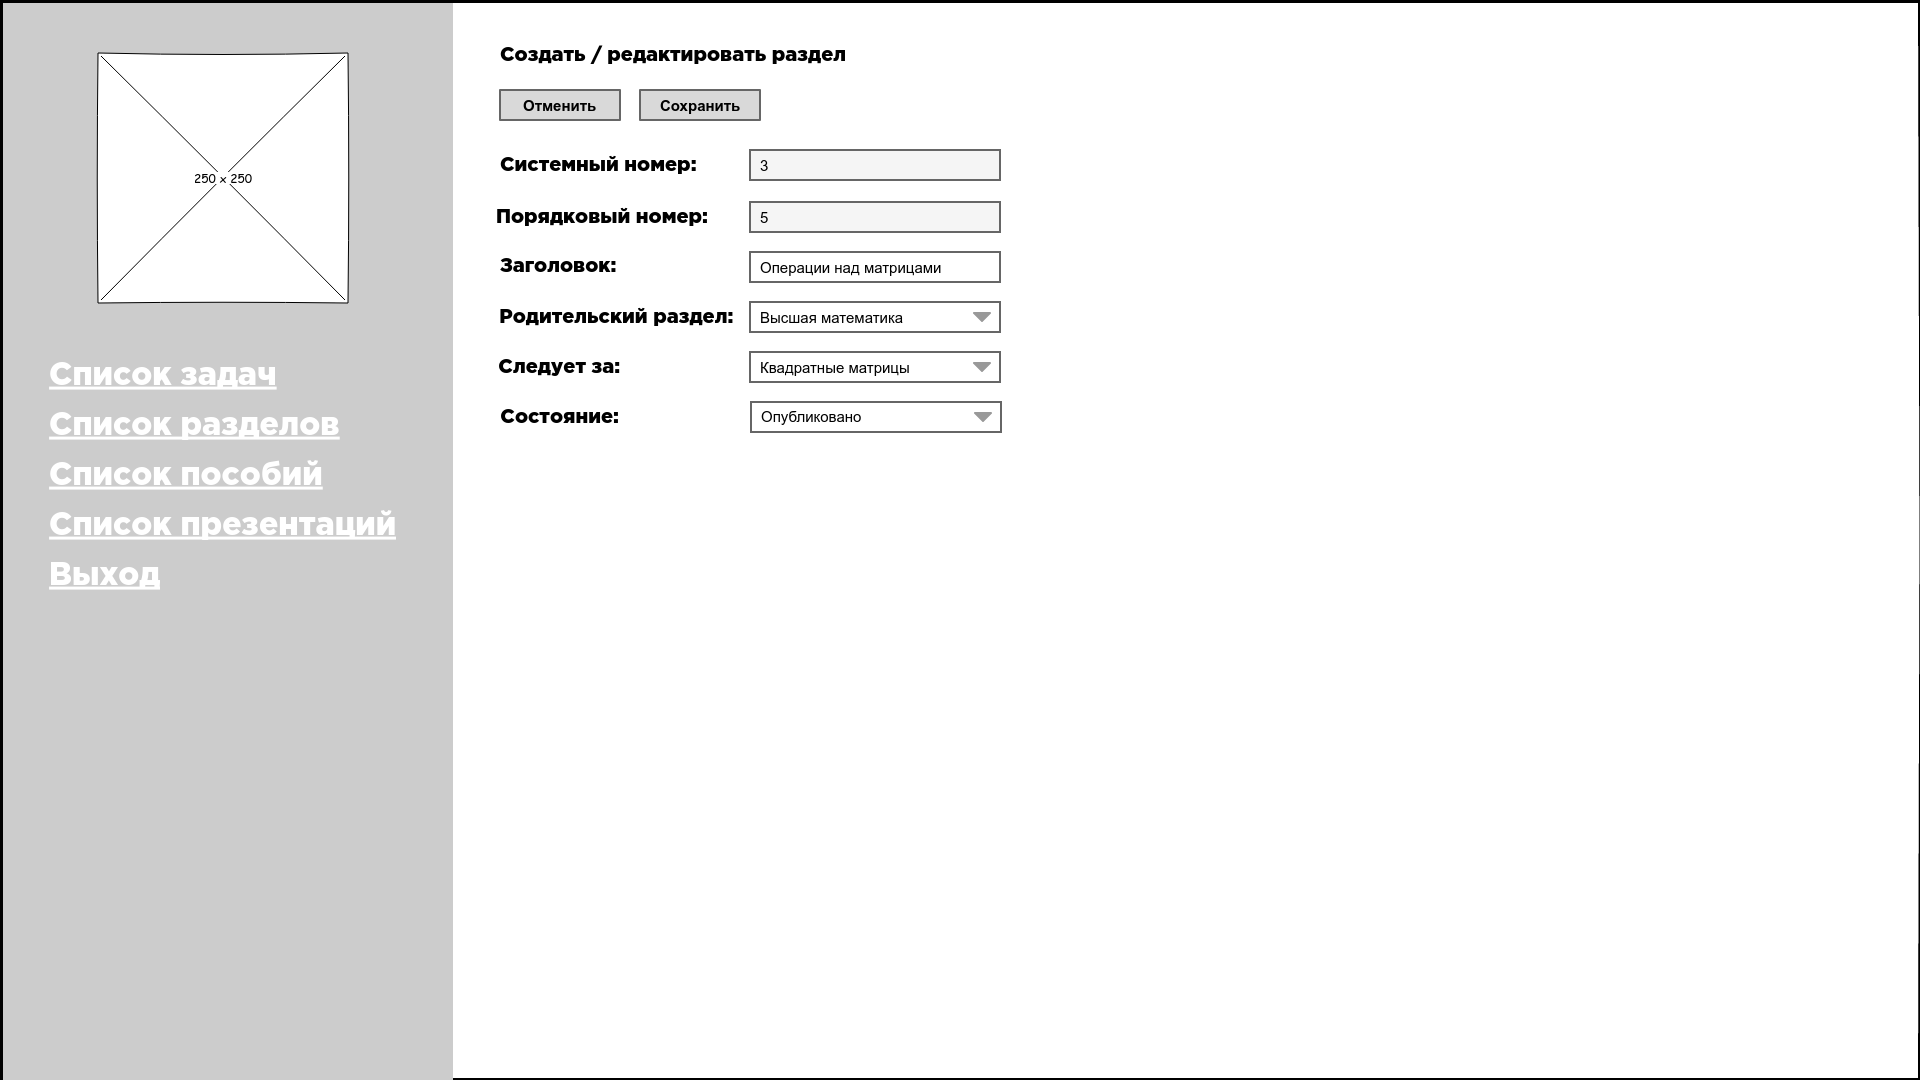
\includegraphics[width=\textwidth]{5-2-3}
\end{figure}
\paragraph{Назначение страницы}
Страница предназначена для создания/редактирования всех разделов из категорий «ЕГЭ профильный уровень», «ЕГЭ базовый уровень», «ОГЭ», «Высшая математика».

\paragraph{Структура страницы}
\begin{enumerate}
	\item Шапка
	\begin{enumerate}
		\item Заголовок
	\end{enumerate}

	\item Меню
	\begin{enumerate}
		\item Логотип
		\item Навигация
	\end{enumerate}

	\item Контент
	\begin{enumerate}
		\item Кнопки управления
		\begin{itemize}
			\item Отменить
			\item Сохранить
		\end{itemize}

		\item Поля редактирования
		\begin{enumerate}
			\item Системный номер
			\item Порядковый номер
			\item Заголовок
			\item Родительский раздел
			\item Следует за
			\item Состояние
		\end{enumerate}
	\end{enumerate}
\end{enumerate}

\paragraph{Функциональные возможности}
\begin{enumerate}
	\item Шапка
	\begin{enumerate}
		\item Заголовок
	\end{enumerate}

	\item Меню
	\begin{enumerate}
		\item Навигация
		\begin{enumerate}
			\item Переход между разделами
		\end{enumerate}
	\end{enumerate}

	\item Контент
	\begin{enumerate}
		\item Кнопки управления
		\begin{itemize}
			\item Отменить
			\begin{enumerate}
				\item Отмена изменений
			\end{enumerate}

			\item Сохранить
			\begin{enumerate}
				\item Сохранение изменений
			\end{enumerate}
		\end{itemize}

		\item Поля редактирования
		\begin{enumerate}
			\item Системный номер
			\begin{itemize}
				\item Отображение системного номер в базе
			\end{itemize}

			\item Порядковый номер
			\begin{itemize}
				\item Изменение порядкового номера раздела
			\end{itemize}

			\item Заголовок
			\begin{itemize}
				\item Изменение заголовка раздела
			\end{itemize}

			\item Родительский раздел
			\begin{itemize}
				\item Выбор родительского раздела
			\end{itemize}

			\item Следует за
			\begin{itemize}
				\item Указание предшествующей задачи
			\end{itemize}

			\item Состояние
			\begin{itemize}
				\item Выбор состояния раздела
			\end{itemize}

		\end{enumerate}
	\end{enumerate}
\end{enumerate}

\subsubsection{Страница «Список задач»}
\begin{figure}[H]
	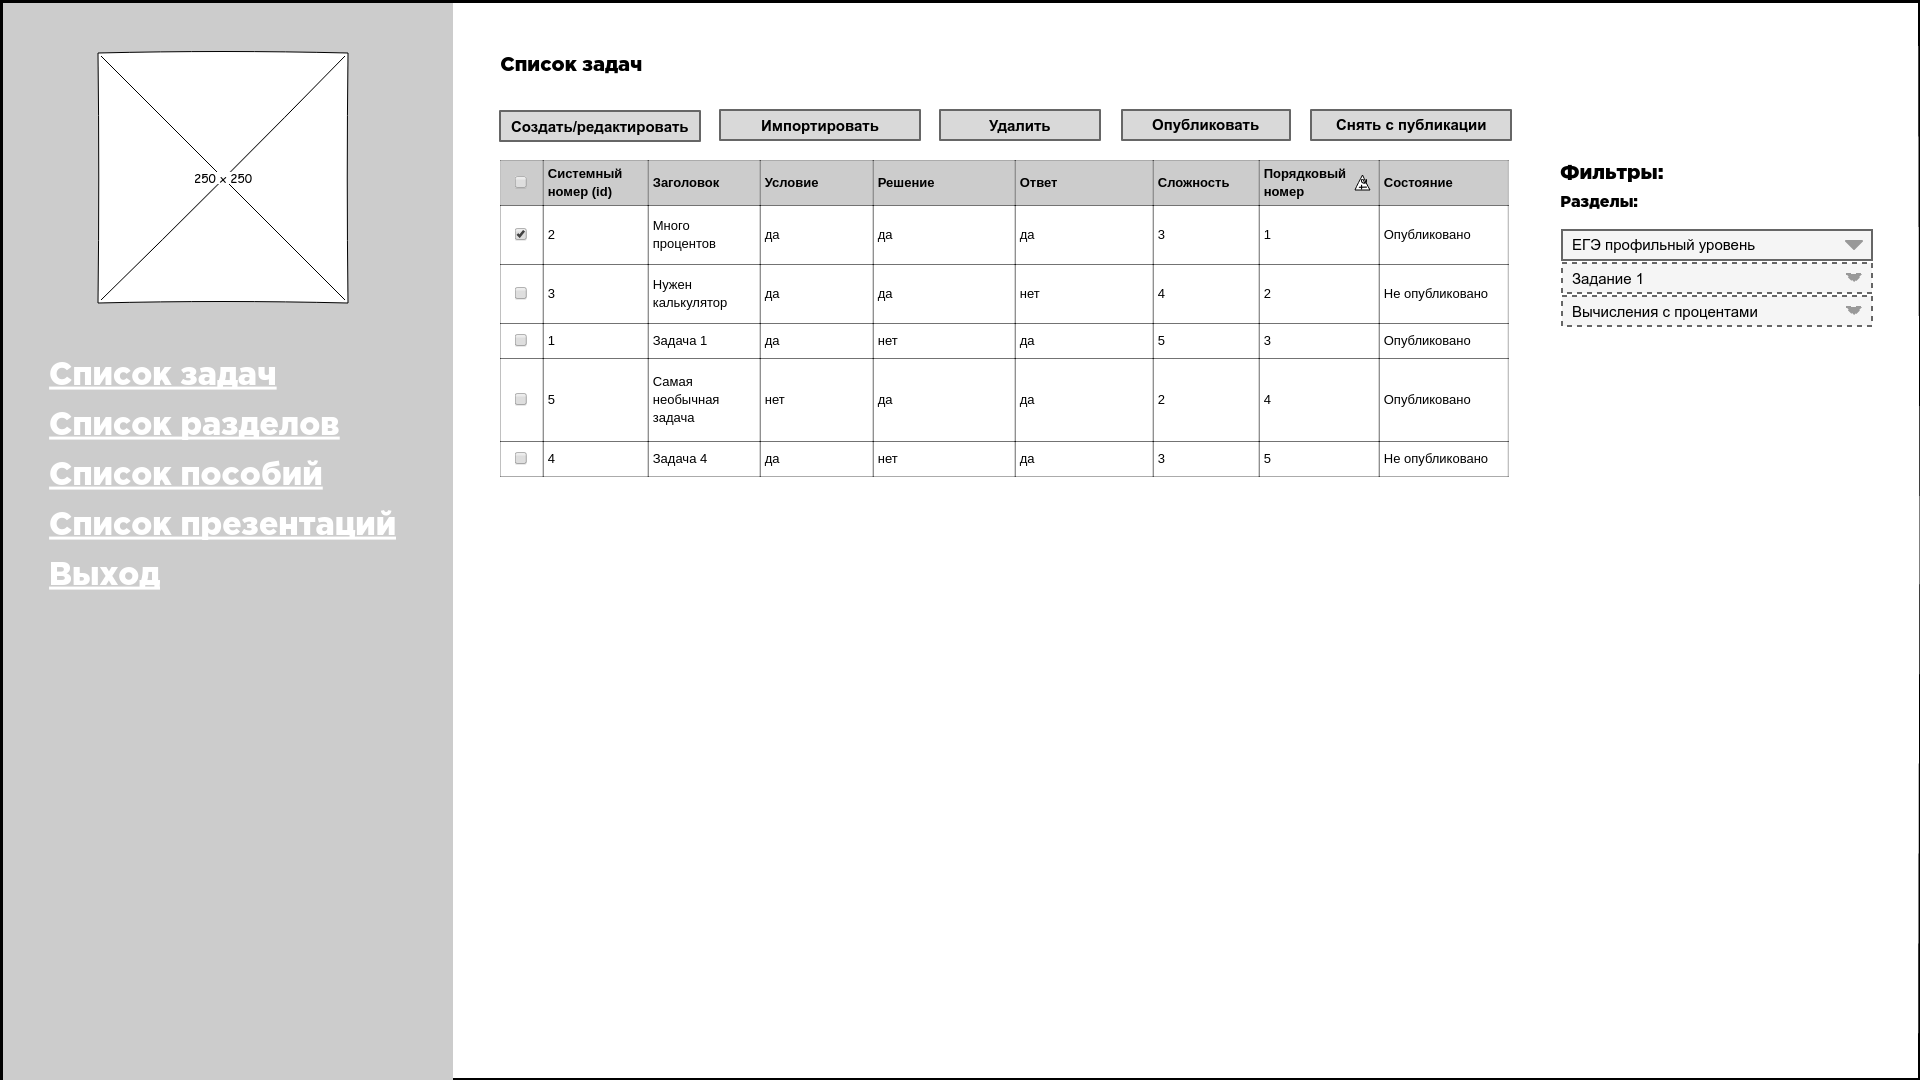
\includegraphics[width=\textwidth]{5-2-4}
\end{figure}
\paragraph{Назначение страницы:} Страница предназначена для управления задачами из категорий «ЕГЭ профильный уровень», «ЕГЭ базовый уровень», «ОГЭ», «Высшая математика».

\paragraph{Структура страницы}
\begin{enumerate}
	\item Шапка
	\begin{enumerate}
		\item Заголовок
	\end{enumerate}

	\item Меню
	\begin{enumerate}
		\item Логотип
		\item Навигация
	\end{enumerate}

	\item Сайдбар
	\begin{enumerate}
		\item Фильтры
		\begin{enumerate}
			\item Разделы
		\end{enumerate}
	\end{enumerate}

	\item Контент
	\begin{enumerate}
		\item Кнопки управления
		\begin{itemize}
			\item Создать/редактировать
			\item Удалить
			\item Импортировать
			\item Опубликовать
			\item Снять с публикации
		\end{itemize}
		\item Таблица задач
	\end{enumerate}
\end{enumerate}

\paragraph{Функциональные возможности}
\begin{enumerate}
	\item Меню
	\begin{enumerate}
		\item Навигация
		\begin{itemize}
			\item Переход между разделами
		\end{itemize}
	\end{enumerate}

	\item Сайдбар
	\begin{enumerate}
		\item Фильтры
		\begin{itemize}
			\item «Фильтрация» задач по разделам
		\end{itemize}
	\end{enumerate}

	\item Контент
	\begin{enumerate}
		\item Таблица разделов
		\begin{itemize}
			\item Сортировка списка разделов по столбцам
		\end{itemize}

		\item Кнопки управления
		\begin{itemize}
			\item Создание задачи
			\item Редактирование задачи
			\item Импорт задачи
			\item Удаление одной или нескольких задач
			\item Изменение состояния задачи на «Опубликовать»
			\item Изменение состояния задачи на «Не опубликовано»
		\end{itemize}
	\end{enumerate}
\end{enumerate}

\subsubsection{Страница «Создать/редактировать задачу»}
\begin{figure}[H]
	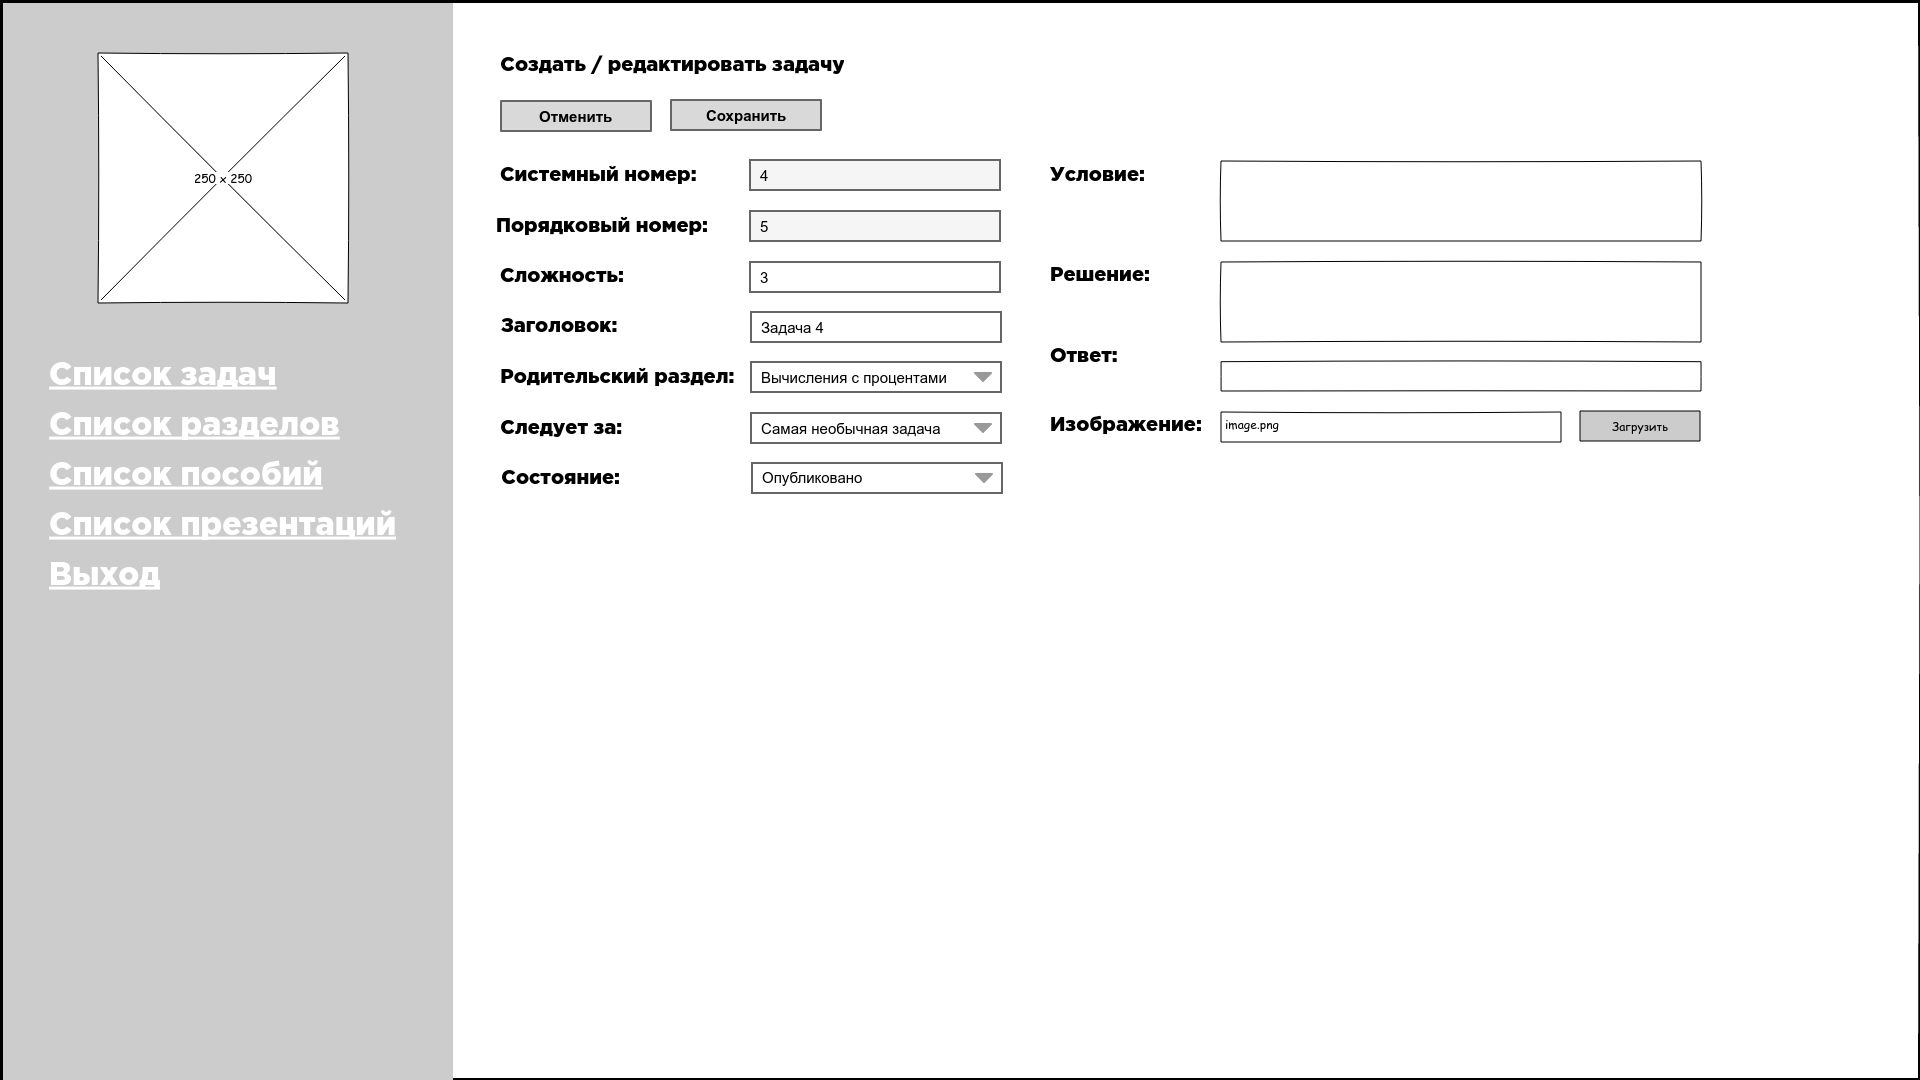
\includegraphics[width=\textwidth]{5-2-5}
\end{figure}
\paragraph{Назначение страницы}
Страница предназначена для создания/редактирования задач из категорий «ЕГЭ профильный уровень», «ЕГЭ базовый уровень», «ОГЭ», «Высшая математика».

\paragraph{Структура страницы}
\begin{enumerate}
	\item Шапка
	\begin{enumerate}
		\item Заголовок
	\end{enumerate}

	\item Меню
	\begin{enumerate}
		\item Логотип
		\item Навигация
	\end{enumerate}

	\item Контент
	\begin{enumerate}
		\item Кнопки управления
		\begin{itemize}
			\item Отменить
			\item Сохранить
		\end{itemize}

		\item Поля редактирования
		\begin{enumerate}
			\item Системный номер
			\item Порядковый номер
			\item Заголовок
			\item Сложность
			\item Родительский раздел
			\item Следует за
			\item Состояние
			\item Условие
			\item Решение
			\item Ответ
			\item Изображение
		\end{enumerate}
	\end{enumerate}
\end{enumerate}

\paragraph{Функциональные возможности}
\begin{enumerate}
	\item Шапка
	\begin{enumerate}
		\item Заголовок
	\end{enumerate}

	\item Меню
	\begin{enumerate}
		\item Навигация
		\begin{enumerate}
			\item Переход между разделами
		\end{enumerate}
	\end{enumerate}

	\item Контент
	\begin{enumerate}
		\item Кнопки управления
		\begin{itemize}
			\item Отменить
			\begin{enumerate}
				\item Отмена изменений
			\end{enumerate}

			\item Сохранить
			\begin{enumerate}
				\item Сохранение изменений
			\end{enumerate}
		\end{itemize}

		\item Поля редактирования
		\begin{enumerate}
			\item Системный номер
			\begin{itemize}
				\item Отображение системного номера в базе
			\end{itemize}

			\item Порядковый номер
			\begin{itemize}
				\item Изменение порядкового номера задачи
			\end{itemize}

			\item Заголовок
			\begin{itemize}
				\item Изменение заголовка задачи
			\end{itemize}

			\item Родительский раздел
			\begin{itemize}
				\item Выбор родительского раздела
			\end{itemize}

			\item Следует за
			\begin{itemize}
				\item Указание предшествующей задачи в списке
			\end{itemize}

			\item Состояние
			\begin{enumerate}
				\item Выбор состояния задачи
			\end{enumerate}

			\item Сложность
			\begin{itemize}
				\item Задание сложности задачи
			\end{itemize}

			\item Условие
			\begin{itemize}
				\item Записать условие задачи
			\end{itemize}

			\item Решение
			\begin{itemize}
				\item Записать решение задачи
			\end{itemize}

			\item Ответ
			\begin{itemize}
				\item Записать ответ задачи
			\end{itemize}

			\item Изображение
			\begin{itemize}
				\item Добавить изображение к задаче
			\end{itemize}

		\end{enumerate}
	\end{enumerate}
\end{enumerate}

\subsubsection{Страница «Импорт задачи»}
\begin{figure}[H]
	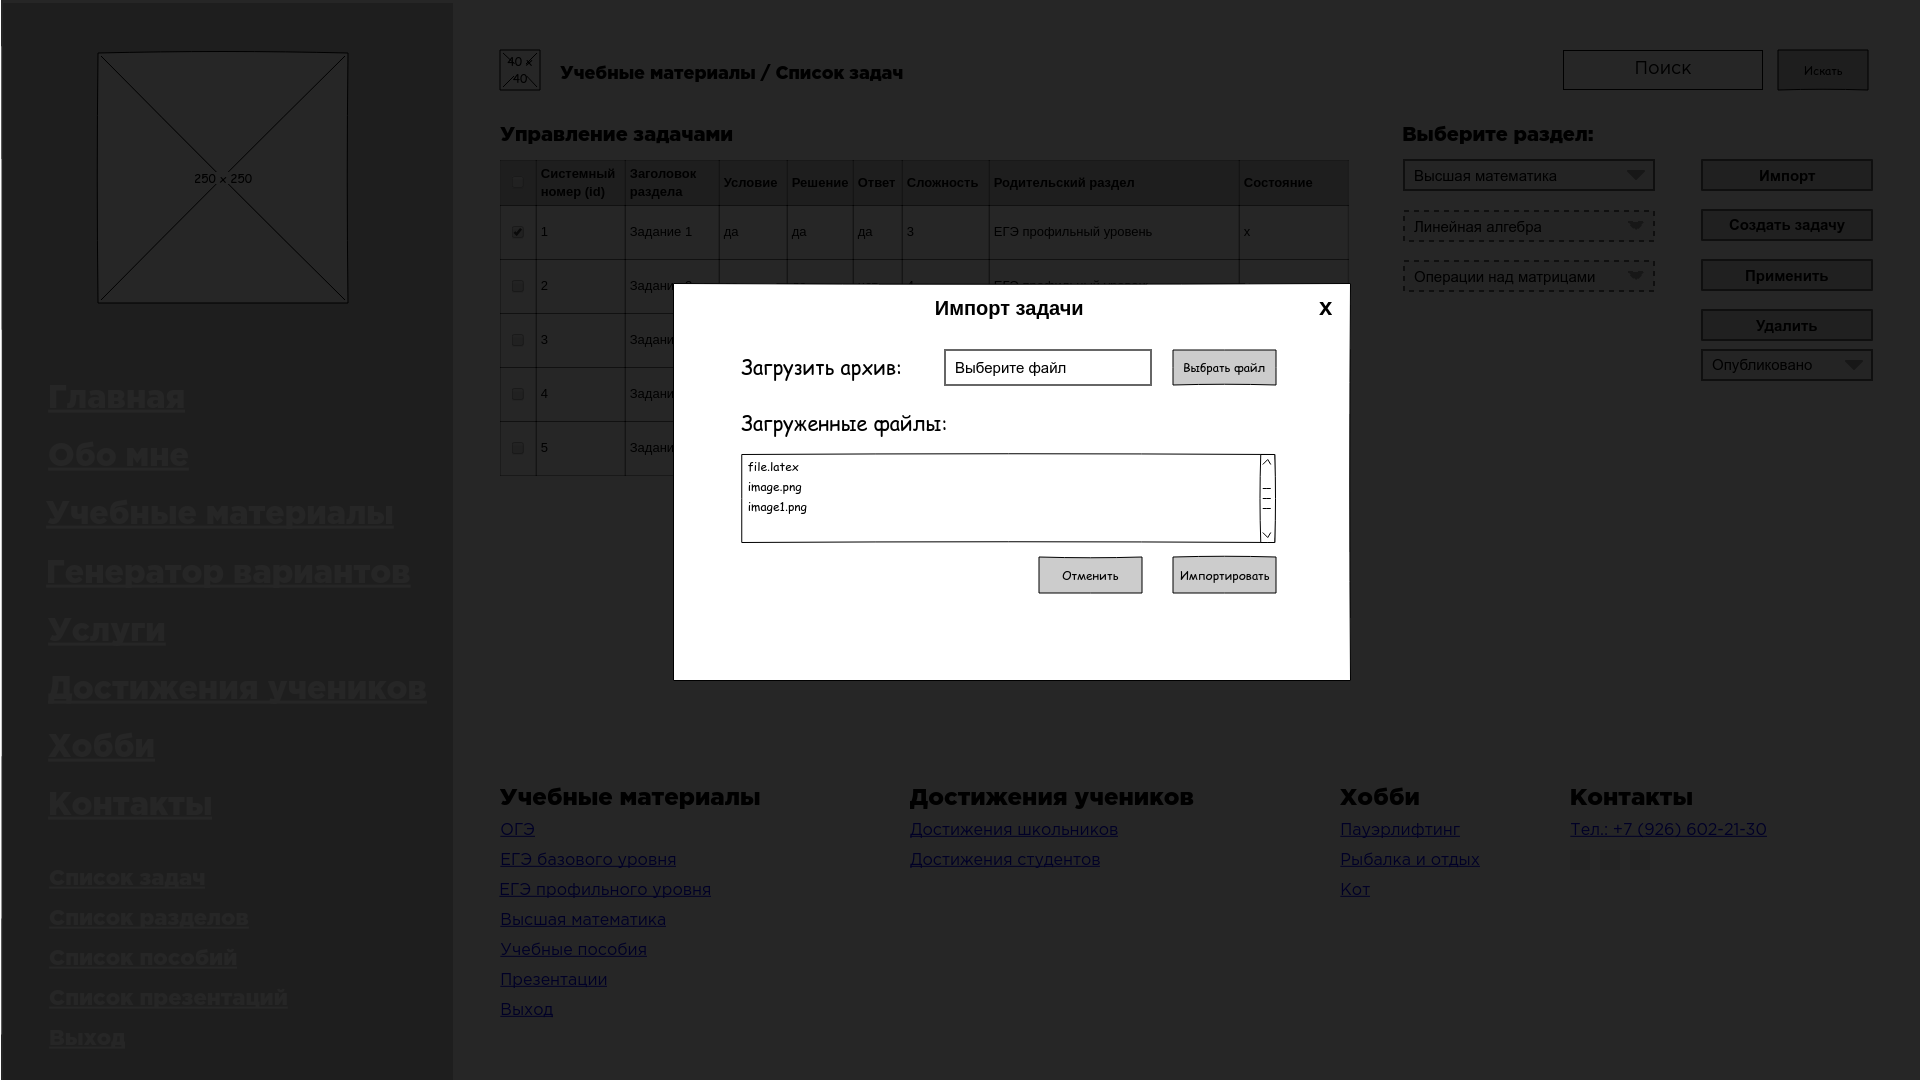
\includegraphics[width=\textwidth]{5-2-6}
\end{figure}
\paragraph{Назначение страницы}
Страница предназначена для импорта задач.

\paragraph{Структура страницы}
\begin{enumerate}
	\item Модальное окно
	\item Кнопки управления
	\begin{enumerate}
		\item Отменить
		\item Импортировать
		\item Закрыть
	\end{enumerate}
\end{enumerate}

\paragraph{Функциональные возможности}
\begin{enumerate}
	\item Модальное окно
	\begin{itemize}
		\item Отображение системного номер в базе
	\end{itemize}
	\item Кнопки управления
	\begin{enumerate}
		\item Отменить
		\begin{itemize}
			\item Отменить импорт
		\end{itemize}

		\item Импортировать
		\begin{itemize}
			\item Импортировать задачу
		\end{itemize}

		\item Закрыть
		\begin{itemize}
			\item Закрыть окно импорта
		\end{itemize}
	\end{enumerate}
\end{enumerate}


\subsubsection{Страница «Список презентаций»}
\begin{figure}[H]
	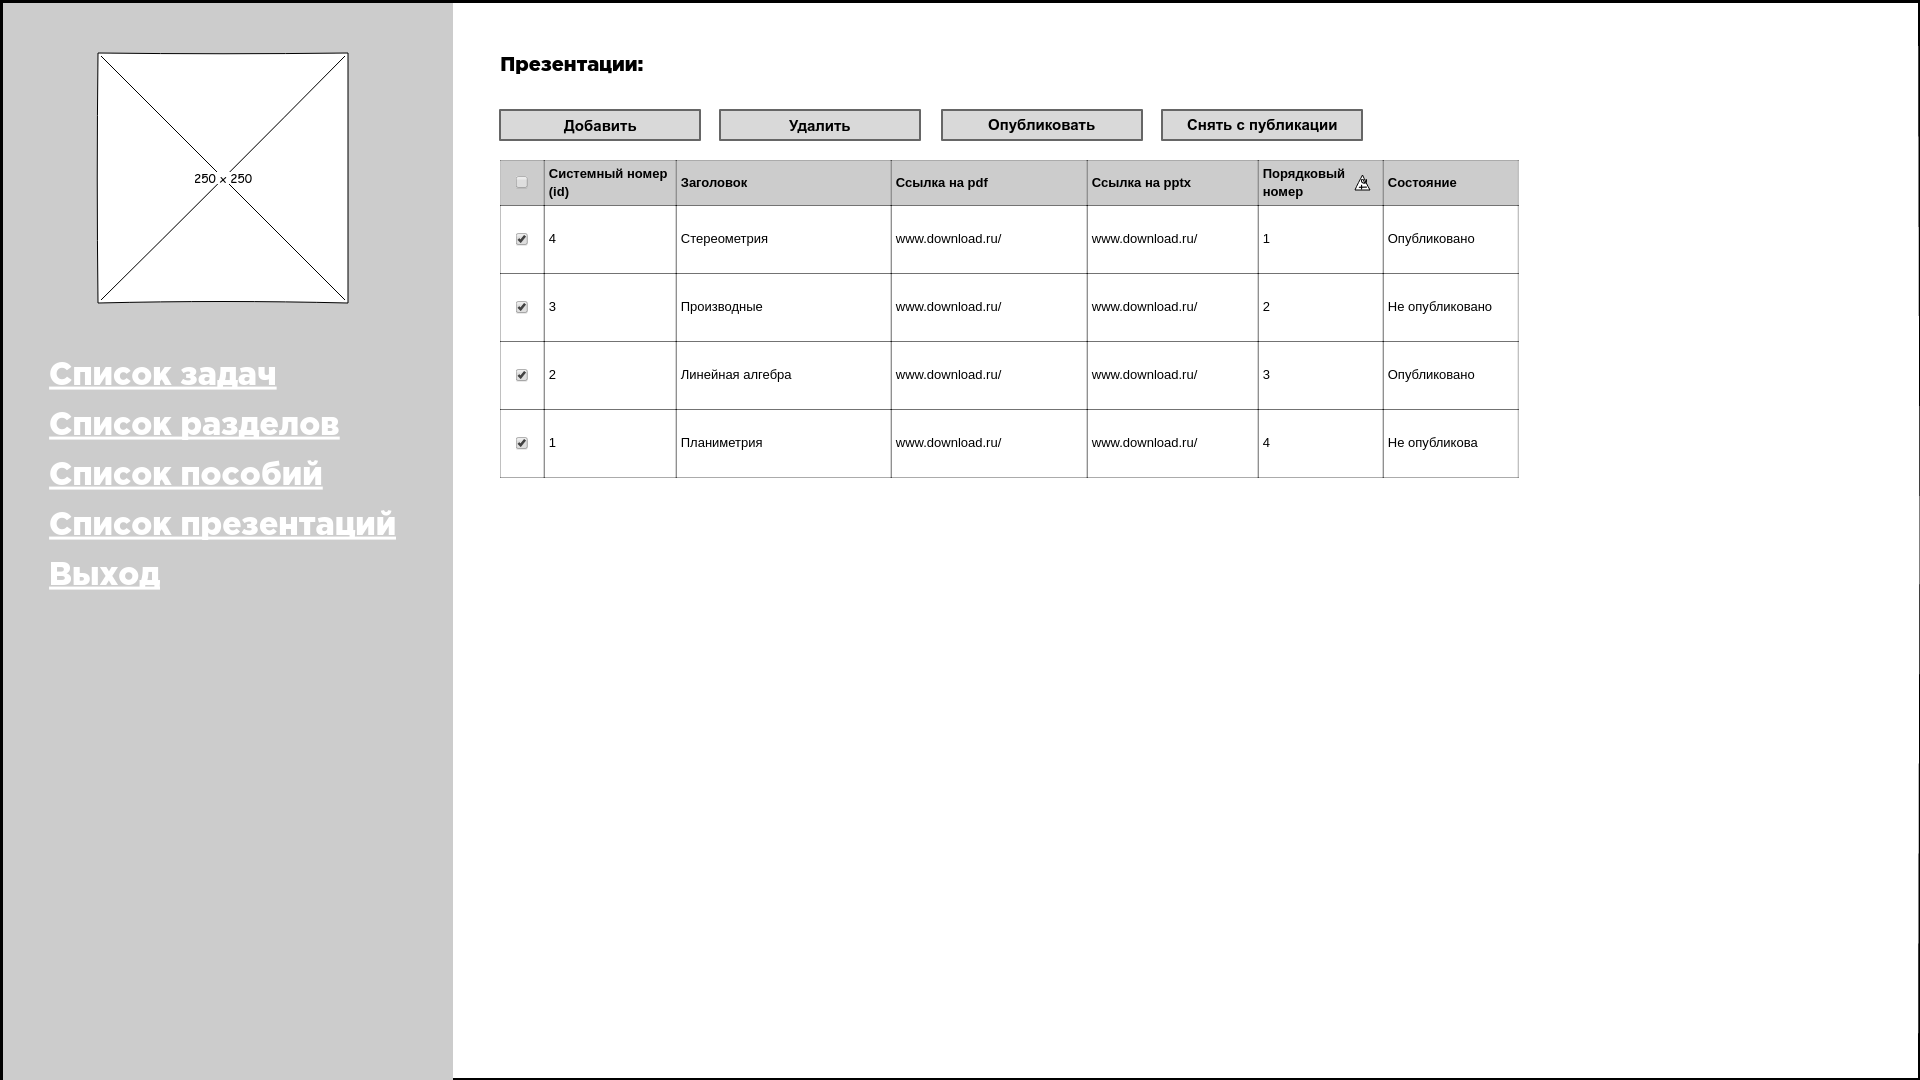
\includegraphics[width=\textwidth]{5-2-7}
\end{figure}
\paragraph{Назначение страницы:} Страница предназначена для управления списком презентаций категории «Презентации».

\paragraph{Структура страницы}
\begin{enumerate}
	\item Шапка
	\begin{enumerate}
		\item Заголовок
	\end{enumerate}

	\item Меню
	\begin{enumerate}
		\item Логотип
		\item Навигация
	\end{enumerate}

	\item Контент
	\begin{enumerate}
		\item Кнопки управления
		\begin{enumerate}
			\item Добавить/редактировать
			\item Удалить
			\item Опубликовать
			\item Снять с публикации
		\end{enumerate}
		\item Таблица презентаций
	\end{enumerate}
\end{enumerate}

\paragraph{Функциональные возможности}
\begin{enumerate}
	\item Меню
	\begin{enumerate}
		\item Навигация
		\begin{itemize}
			\item Переход между разделами
		\end{itemize}
	\end{enumerate}

	\item Контент
	\begin{enumerate}
		\item Таблица презентаций
		\begin{itemize}
			\item Сортировка списка презентаций по столбцам
		\end{itemize}

		\item Кнопки управления
		\begin{itemize}
			\item Добавление/редактирование презентации
			\item Удаление одной или нескольких презентаций
		\end{itemize}
	\end{enumerate}
\end{enumerate}


\subsubsection{Страница «Добавить/редактировать презентацию»}
\begin{figure}[H]
	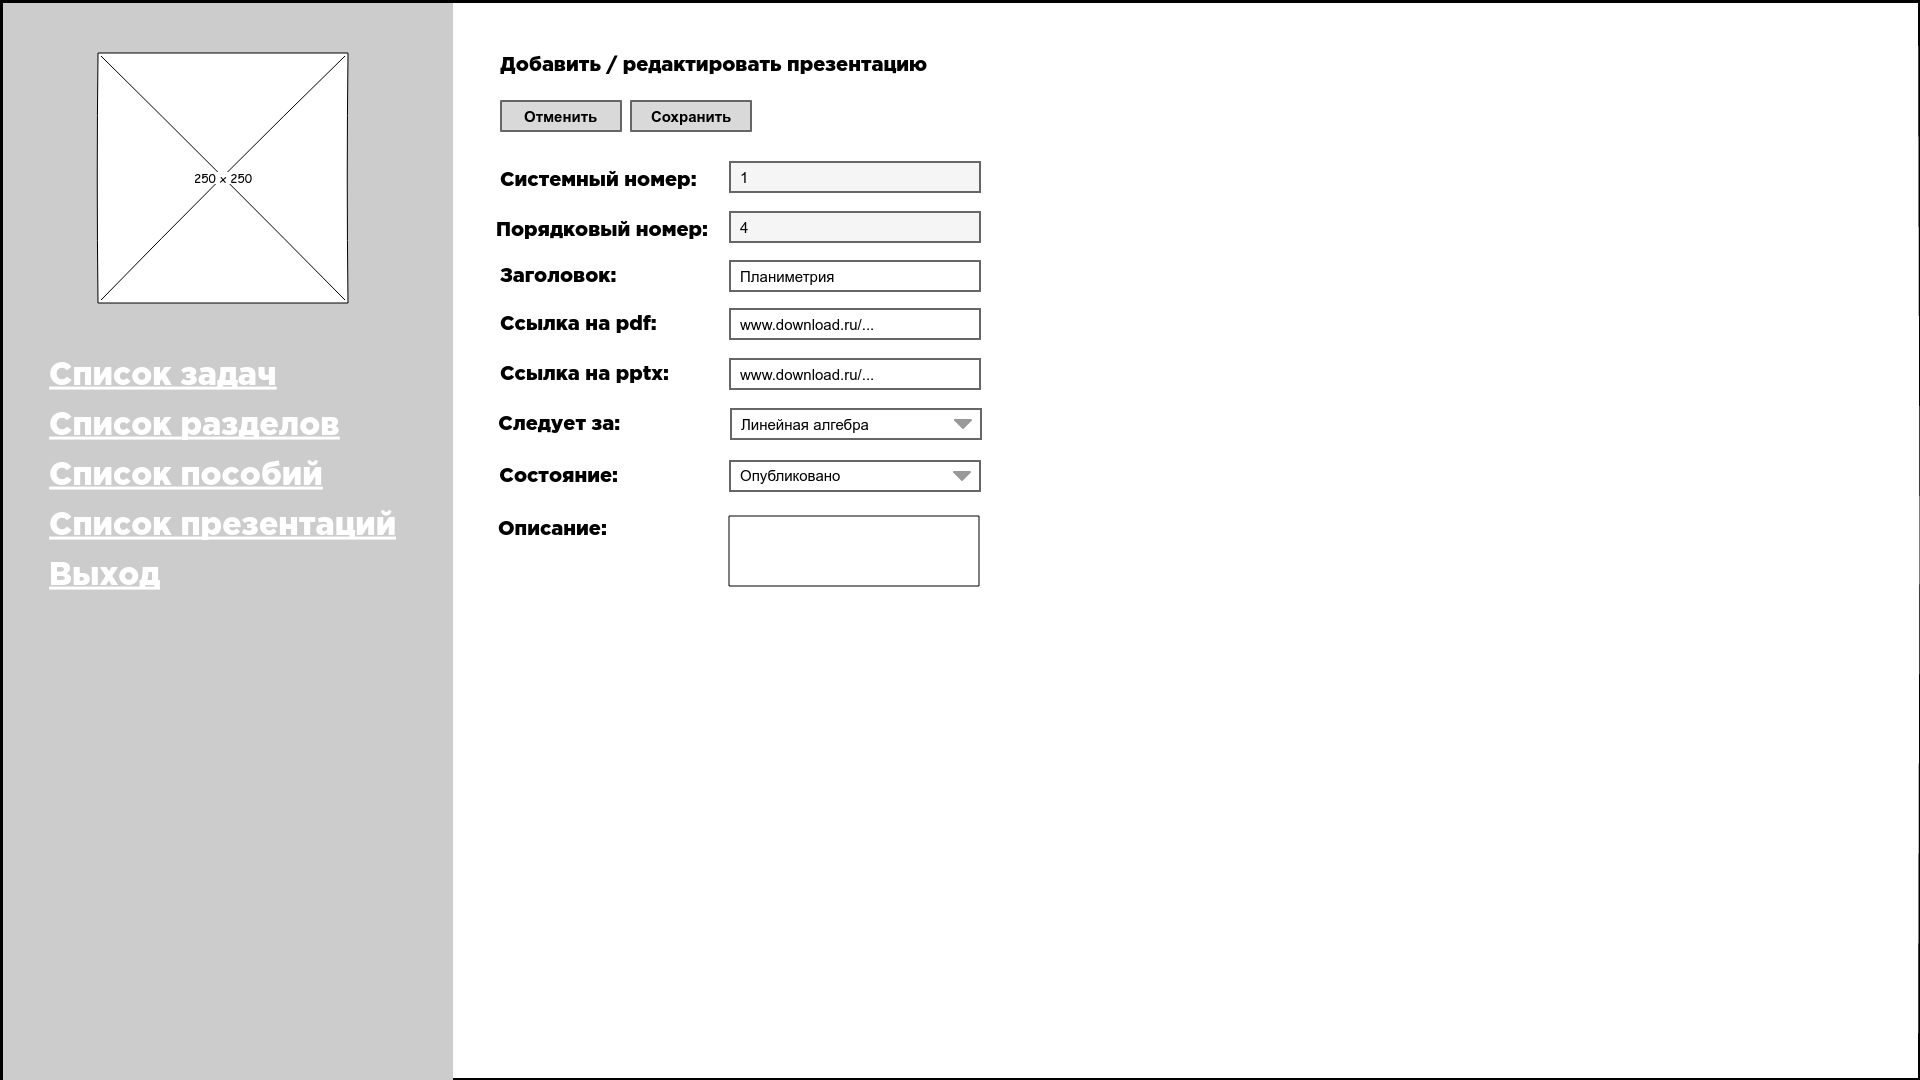
\includegraphics[width=\textwidth]{5-2-8}
\end{figure}
\paragraph{Назначение страницы:} Страница предназначена для обеспечения возможности добавления и редактирования презентаций.

\paragraph{Структура страницы}
\begin{enumerate}
	\item Шапка
	\begin{enumerate}
		\item Заголовок
	\end{enumerate}

	\item Меню
	\begin{enumerate}
		\item Логотип
		\item Навигация
	\end{enumerate}

	\item Контент
	\begin{enumerate}
		\item Кнопки управления
		\begin{itemize}
			\item Отменить
			\item Сохранить
		\end{itemize}
		\item Поля редактирования
		\begin{itemize}
			\item Системный номер
			\item Порядковый номер
			\item Заголовок
			\item Ссылка на pdf
			\item Ссылка на pptx
			\item Следует за
			\item Состояние
			\item Описание
		\end{itemize}
	\end{enumerate}
\end{enumerate}

\paragraph{Функциональные возможности}
\begin{enumerate}
	\item Меню
	\begin{enumerate}
		\item Навигация
		\begin{itemize}
			\item Переход между разделами
		\end{itemize}
	\end{enumerate}

	\item Контент
	\begin{enumerate}
		\item Кнопки управления
		\begin{itemize}
			\item Отмена изменений
			\item Сохранение изменений
		\end{itemize}

		\item Поля редактирования
		\begin{enumerate}
			\item Системный номер
			\begin{itemize}
				\item Отображение системного номера в базе
			\end{itemize}

			\item Порядковый номер
			\begin{itemize}
				\item Изменение порядкового номера презентации
			\end{itemize}

			\item Заголовок
			\begin{itemize}
				\item Изменение заголовка задачи
			\end{itemize}

			\item Ссылка на pdf
			\begin{itemize}
				\item Добавление ссылки на скачивание презентации в формате pdf
			\end{itemize}

			\item Ссылка на pptx
			\begin{itemize}
				\item Добавление ссылки на скачивание презентации в формате pptx
			\end{itemize}

			\item Следует за
			\begin{itemize}
				\item Указание предшествующей презентации в списке
			\end{itemize}

			\item Состояние
			\begin{itemize}
				\item Выбор состояния презентации
			\end{itemize}

			\item Описание
			\begin{itemize}
				\item Добавление описания презентации
			\end{itemize}


		\end{enumerate}
	\end{enumerate}
\end{enumerate}


\subsubsection{Страница «Список пособий»}
\begin{figure}[H]
	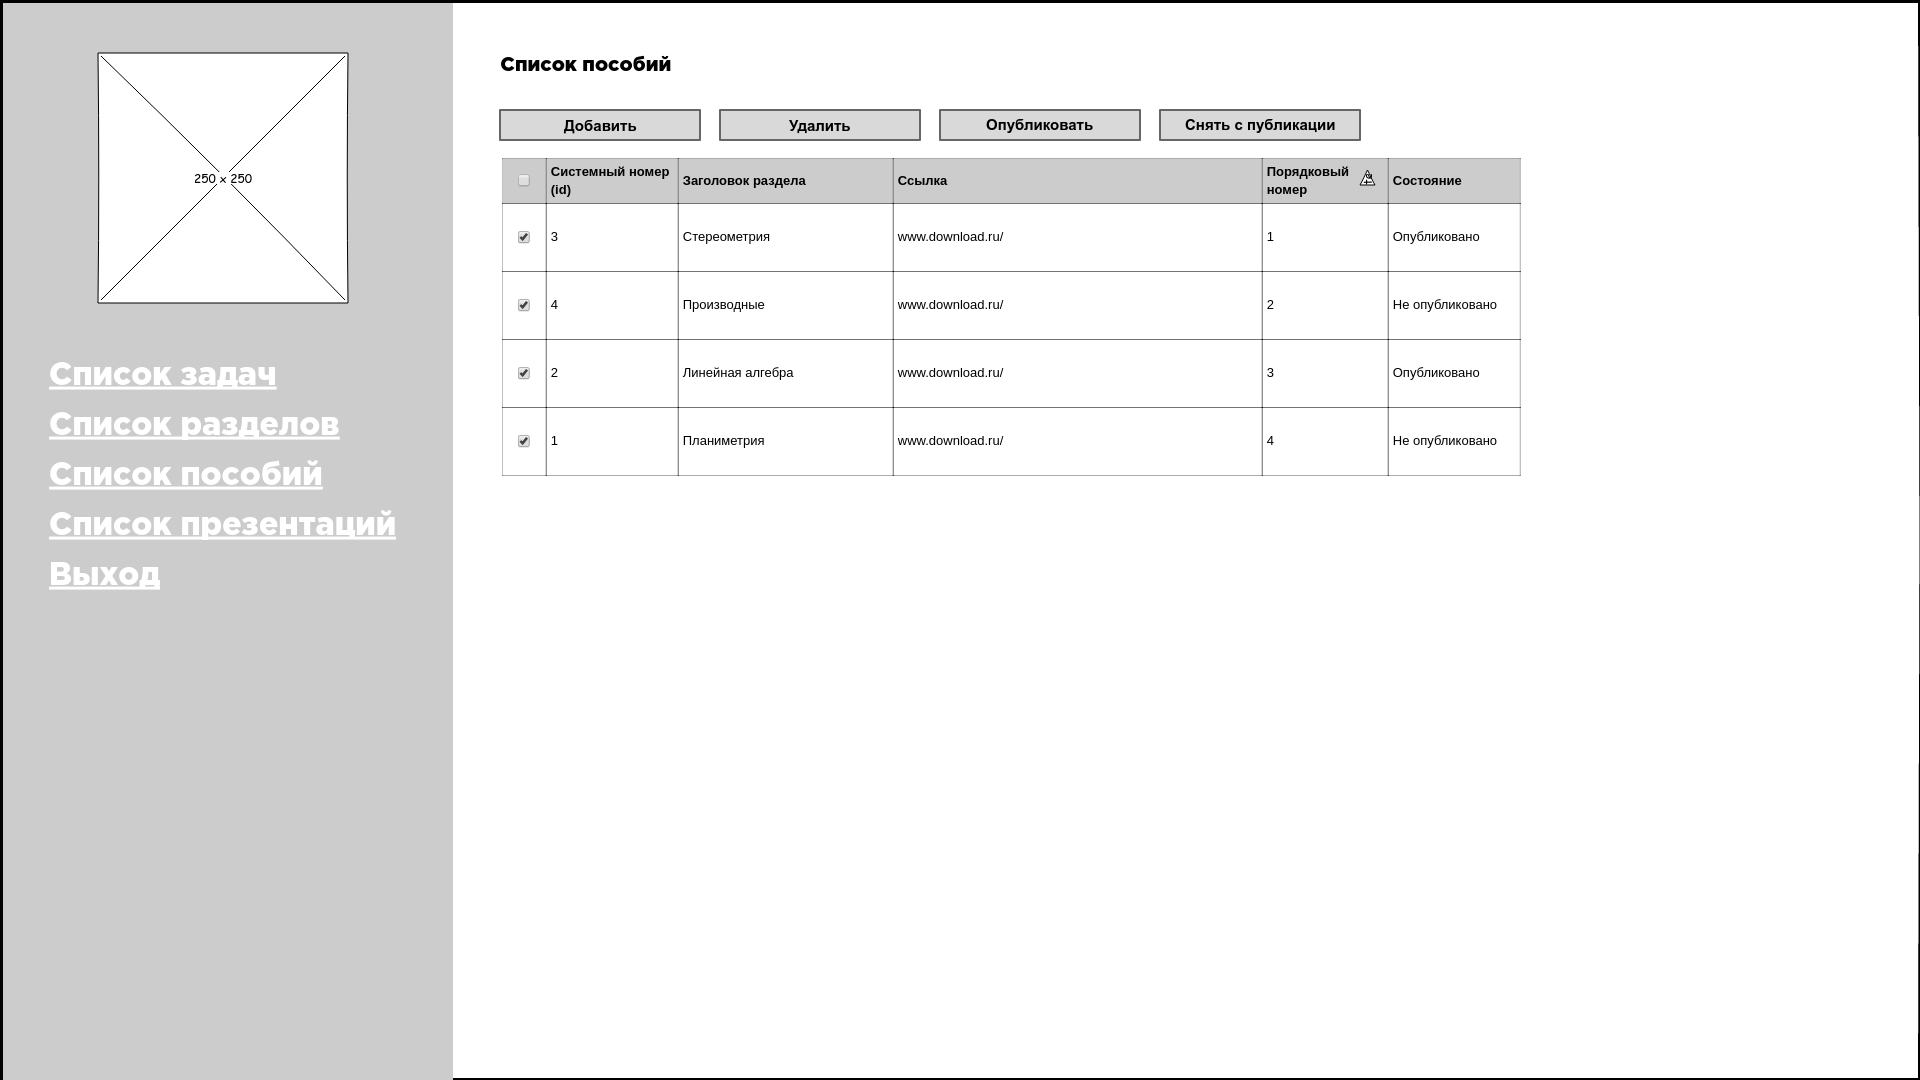
\includegraphics[width=\textwidth]{5-2-9}
\end{figure}
\paragraph{Назначение страницы:} Страница предназначена для управления списком пособий категории «Учебные пособия».

\paragraph{Структура страницы}
\begin{enumerate}
	\item Шапка
	\begin{enumerate}
		\item Заголовок
	\end{enumerate}

	\item Меню
	\begin{enumerate}
		\item Логотип
		\item Навигация
	\end{enumerate}

	\item Контент
	\begin{enumerate}
		\item Кнопки управления
		\begin{itemize}
			\item Добавить/редактировать
			\item Удалить
			\item Опубликовать
			\item Снять с публикации
		\end{itemize}
		\item Таблица пособий
	\end{enumerate}
\end{enumerate}

\paragraph{Функциональные возможности}
\begin{enumerate}
	\item Меню
	\begin{enumerate}
		\item Навигация
		\begin{itemize}
			\item Переход между разделами
		\end{itemize}
	\end{enumerate}

	\item Контент
	\begin{enumerate}
		\item Таблица пособий
		\begin{itemize}
			\item Сортировка списка пособий по столбцам
		\end{itemize}

		\item Кнопки управления
		\begin{itemize}
			\item Создание/редактирование презентации
			\item Удаление одной или нескольких презентаций
			\item Публикация одной или нескольких презентаций
			\item Снятие одной или нескольких презентаций с публикации
		\end{itemize}
	\end{enumerate}
\end{enumerate}


\subsubsection{Страница «Добавить/редактировать пособие»}
\begin{figure}[H]
	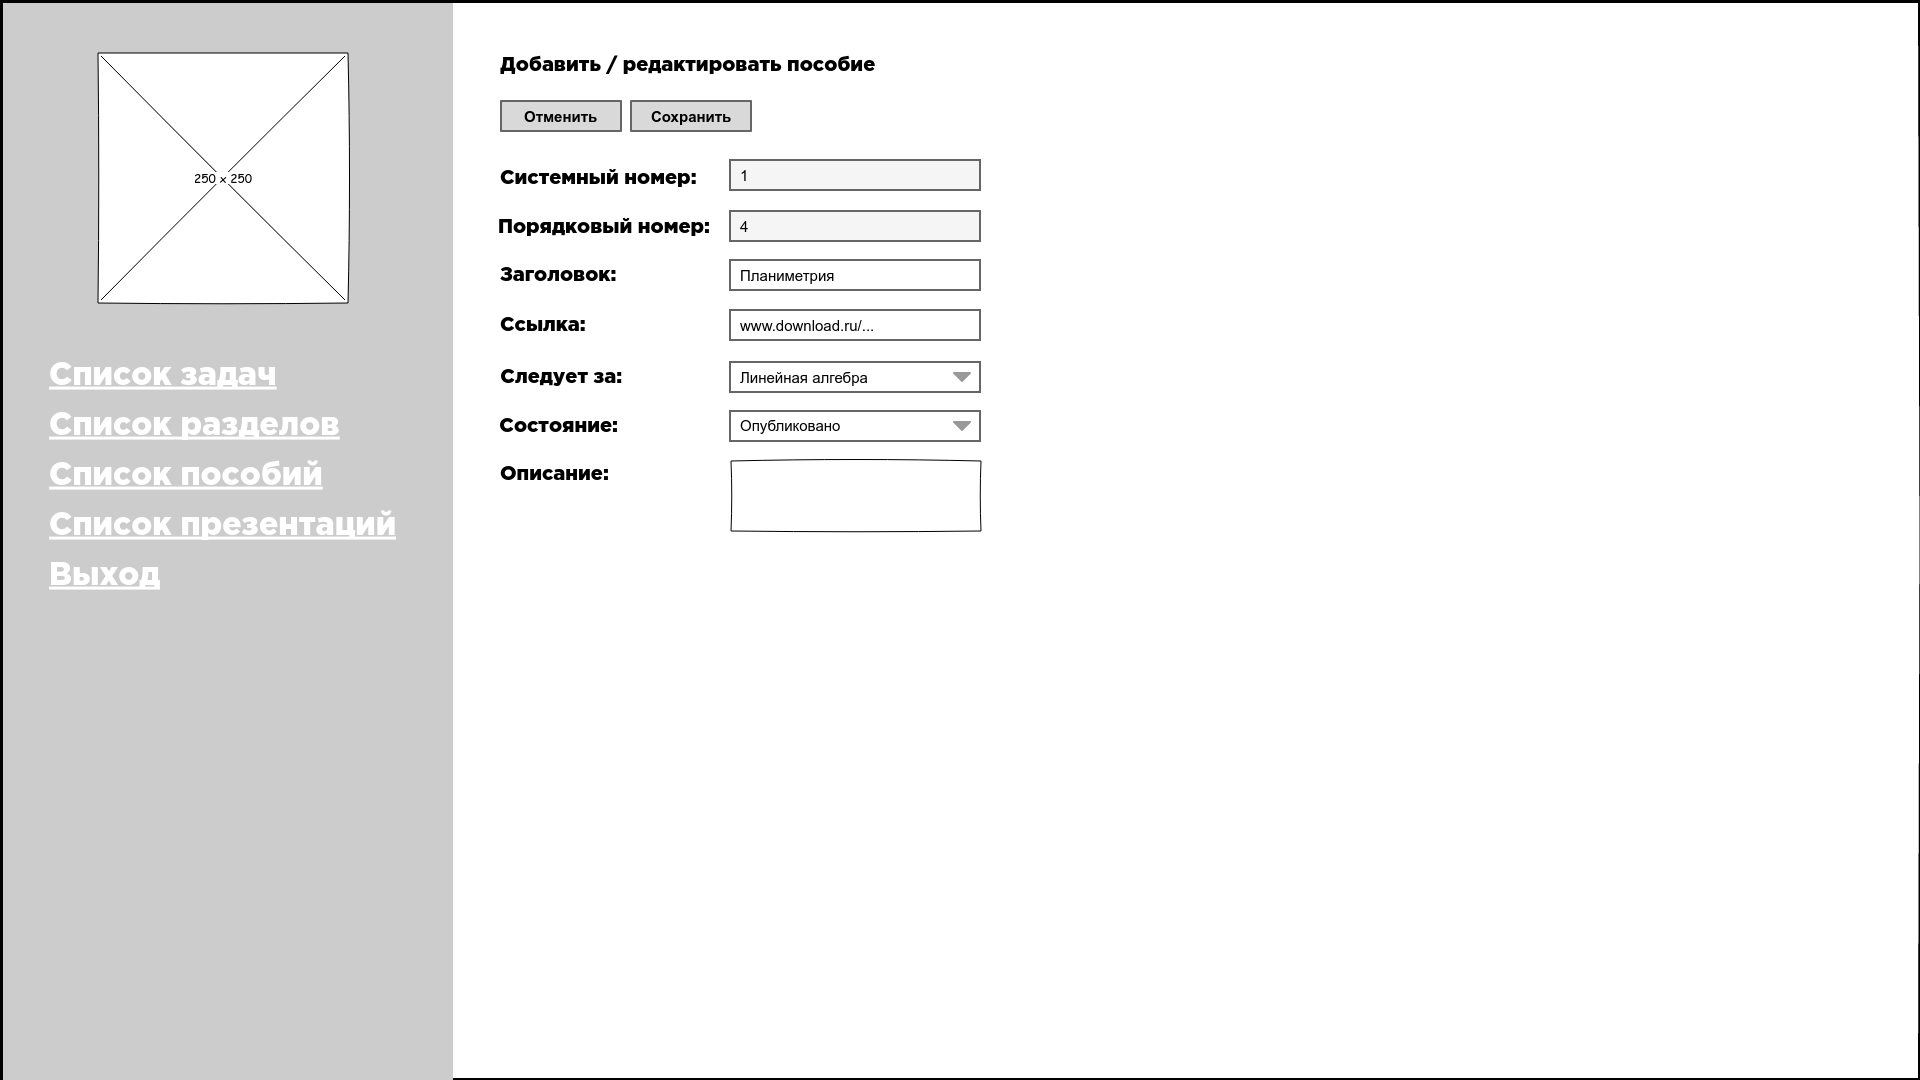
\includegraphics[width=\textwidth]{5-2-10}
\end{figure}
\paragraph{Назначение страницы:} Страница предназначена для обеспечения возможности добавления и редактирования учебных пособий.

\paragraph{Структура страницы}
\begin{enumerate}
	\item Шапка
	\begin{enumerate}
		\item Заголовок
	\end{enumerate}

	\item Меню
	\begin{enumerate}
		\item Логотип
		\item Навигация
	\end{enumerate}

	\item Контент
	\begin{enumerate}
		\item Кнопки управления
		\begin{itemize}
			\item Отменить
			\item Сохранить
		\end{itemize}
		\item Поля редактирования
		\begin{itemize}
			\item Системный номер
			\item Порядковый номер
			\item Заголовок
			\item Ссылка на pdf
			\item Следует за
			\item Состояние
			\item Описание
		\end{itemize}
	\end{enumerate}
\end{enumerate}

\paragraph{Функциональные возможности}
\begin{enumerate}
	\item Меню
	\begin{enumerate}
		\item Навигация
		\begin{itemize}
			\item Переход между разделами
		\end{itemize}
	\end{enumerate}

	\item Контент
	\begin{enumerate}
		\item Кнопки управления
		\begin{itemize}
			\item Отмена изменений
			\item Сохранение изменений
		\end{itemize}

		\item Поля редактирования
		\begin{enumerate}
			\item Системный номер
			\begin{itemize}
				\item Отображение системного номера в базе
			\end{itemize}

			\item Порядковый номер
			\begin{itemize}
				\item Изменение порядкового номера пособия
			\end{itemize}

			\item Заголовок
			\begin{itemize}
				\item Изменение заголовка пособия
			\end{itemize}

			\item Ссылка на pdf
			\begin{itemize}
				\item Добавление ссылки на скачивание пособия в формате pdf
			\end{itemize}

			\item Следует за
			\begin{itemize}
				\item Указание предшествующей пособия в списке
			\end{itemize}

			\item Состояние
			\begin{itemize}
				\item Выбор состояния пособия
			\end{itemize}

			\item Описание
			\begin{itemize}
				\item Добавление описания пособия
			\end{itemize}

		\end{enumerate}
	\end{enumerate}
\end{enumerate}


\subsection{Описание страниц. Клиентская часть}

\subsubsection{Страница «Содержание»}
\begin{figure}[H]
	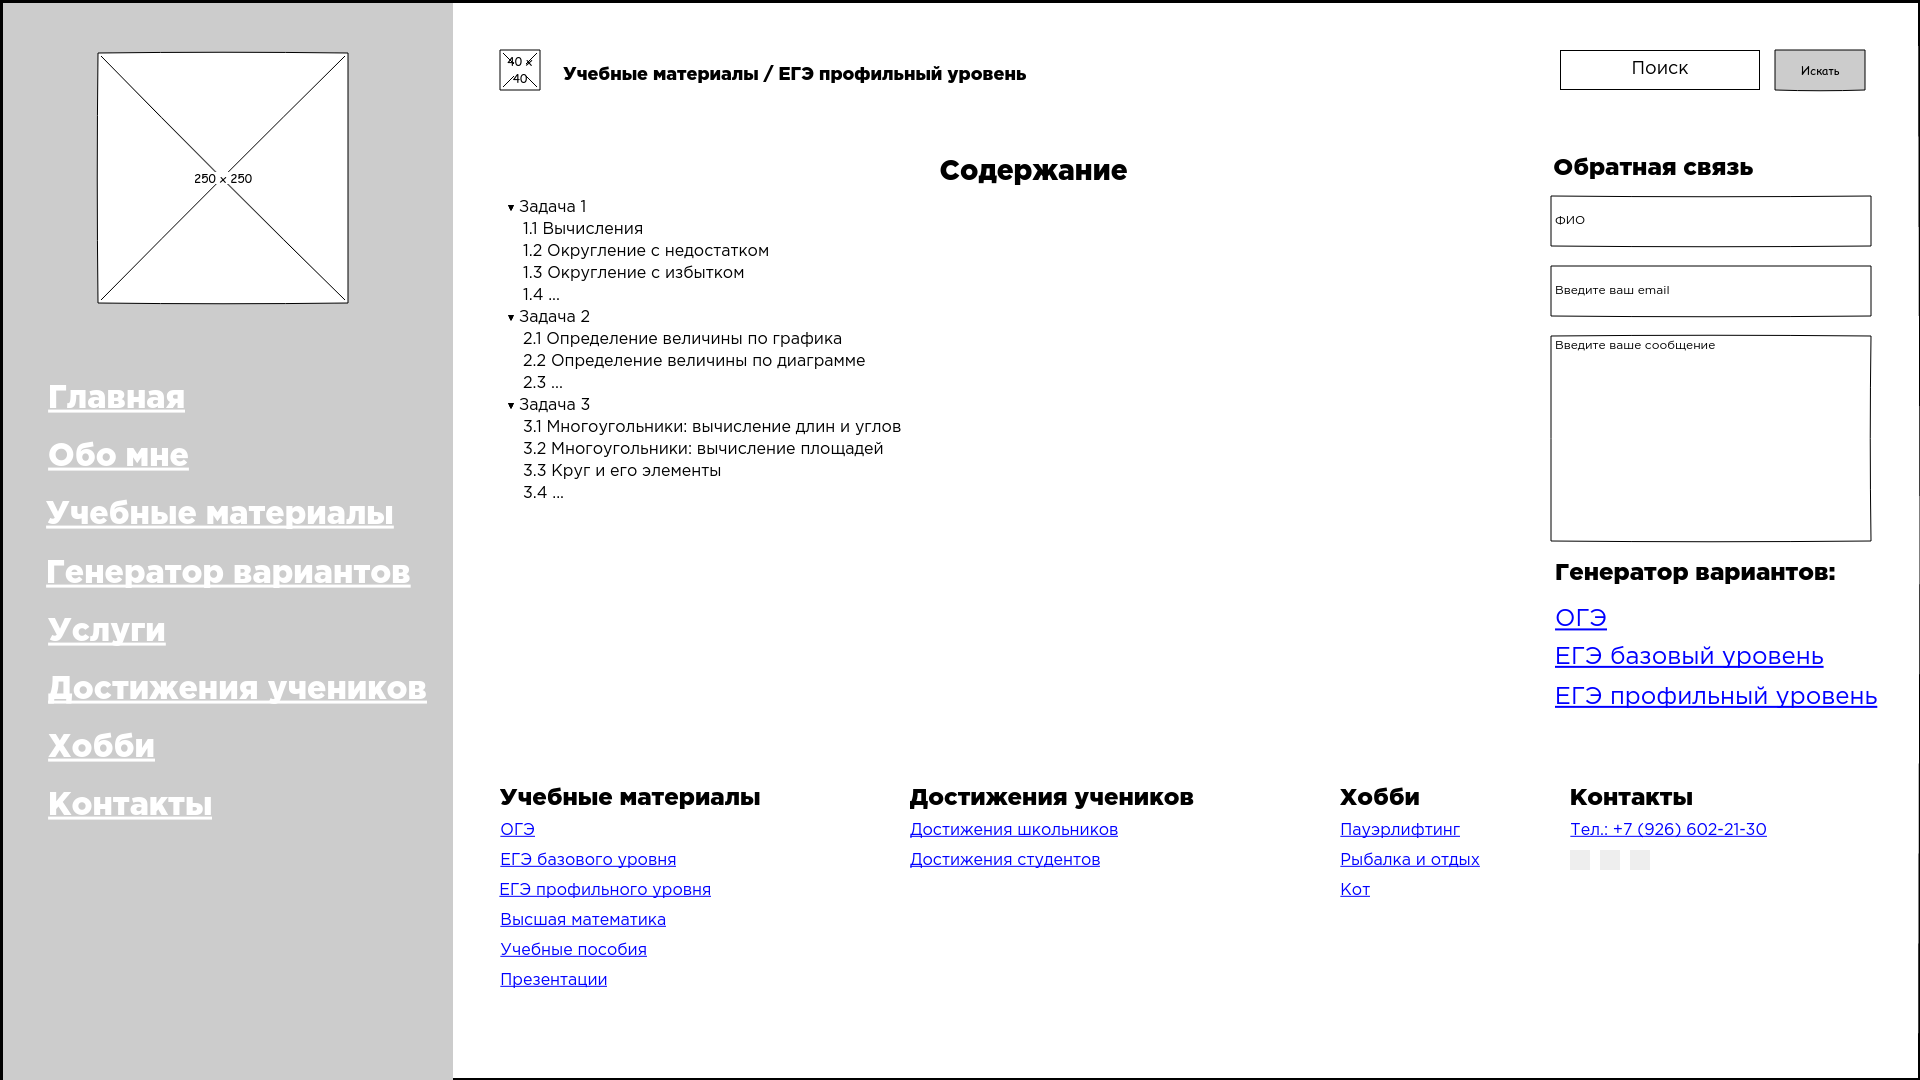
\includegraphics[width=\textwidth]{5-3-1}
\end{figure}

\paragraph{Назначение страницы:} Страница предназначена для удобной навигации по разделам категорий «ЕГЭ профильный уровень», «ЕГЭ базовый уровень», «ОГЭ», «Высшая математика».

\paragraph{Структура страницы}
\begin{enumerate}
	\item Шапка
	\begin{enumerate}
		\item «Хлебные крошки»
		\item Поиск
	\end{enumerate}

	\item Меню
	\begin{enumerate}
		\item Логотип
		\item Навигация
	\end{enumerate}

	\item Сайдбар
	\begin{enumerate}
		\item Форма обратной связи
		\item Ссылки на социальные сети
		\item Генератор вариантов
	\end{enumerate}

	\item Контент
	\begin{enumerate}
		\item Содержание
	\end{enumerate}

	\item Футер
	\begin{enumerate}
		\item Навигация
	\end{enumerate}
\end{enumerate}

\paragraph{Функциональные возможности}
\begin{enumerate}

	\item Шапка
	\begin{enumerate}
		\item «Хлебные крошки»
		\begin{itemize}
			\item Навигация по разделам сайта
		\end{itemize}
		\item Поиск
		\begin{itemize}
			\item Поиск по сайту
		\end{itemize}
	\end{enumerate}

	\item Меню
	\begin{enumerate}
		\item Навигация
		\begin{itemize}
			\item Переход между разделами
		\end{itemize}
	\end{enumerate}

	\item Сайдбар
	\begin{enumerate}
		\item Форма обратной связи
		\begin{itemize}
			\item Отправка сообщений администрации сайта
		\end{itemize}

		\item Ссылки на социальные сети
		\begin{itemize}
			\item Переход на страницы социальных
		\end{itemize}

		\item Генератор вариантов
		\begin{itemize}
			\item Переход в раздел «Генератор вариантов»
		\end{itemize}
	\end{enumerate}

	\item Контент
	\begin{enumerate}
		\item Содержание
		\begin{itemize}
			\item Навигация по разделам категорий «ЕГЭ профильный уровень», «ЕГЭ базовый уровень», «ОГЭ», «Высшая математика»
		\end{itemize}
	\end{enumerate}

	\item Футер
	\begin{enumerate}
		\item Навигация
		\begin{itemize}
			\item Дополнительная навигация по сайту
		\end{itemize}
	\end{enumerate}
\end{enumerate}


\subsubsection{Страница «Генератор вариантов»}
\begin{figure}[H]
	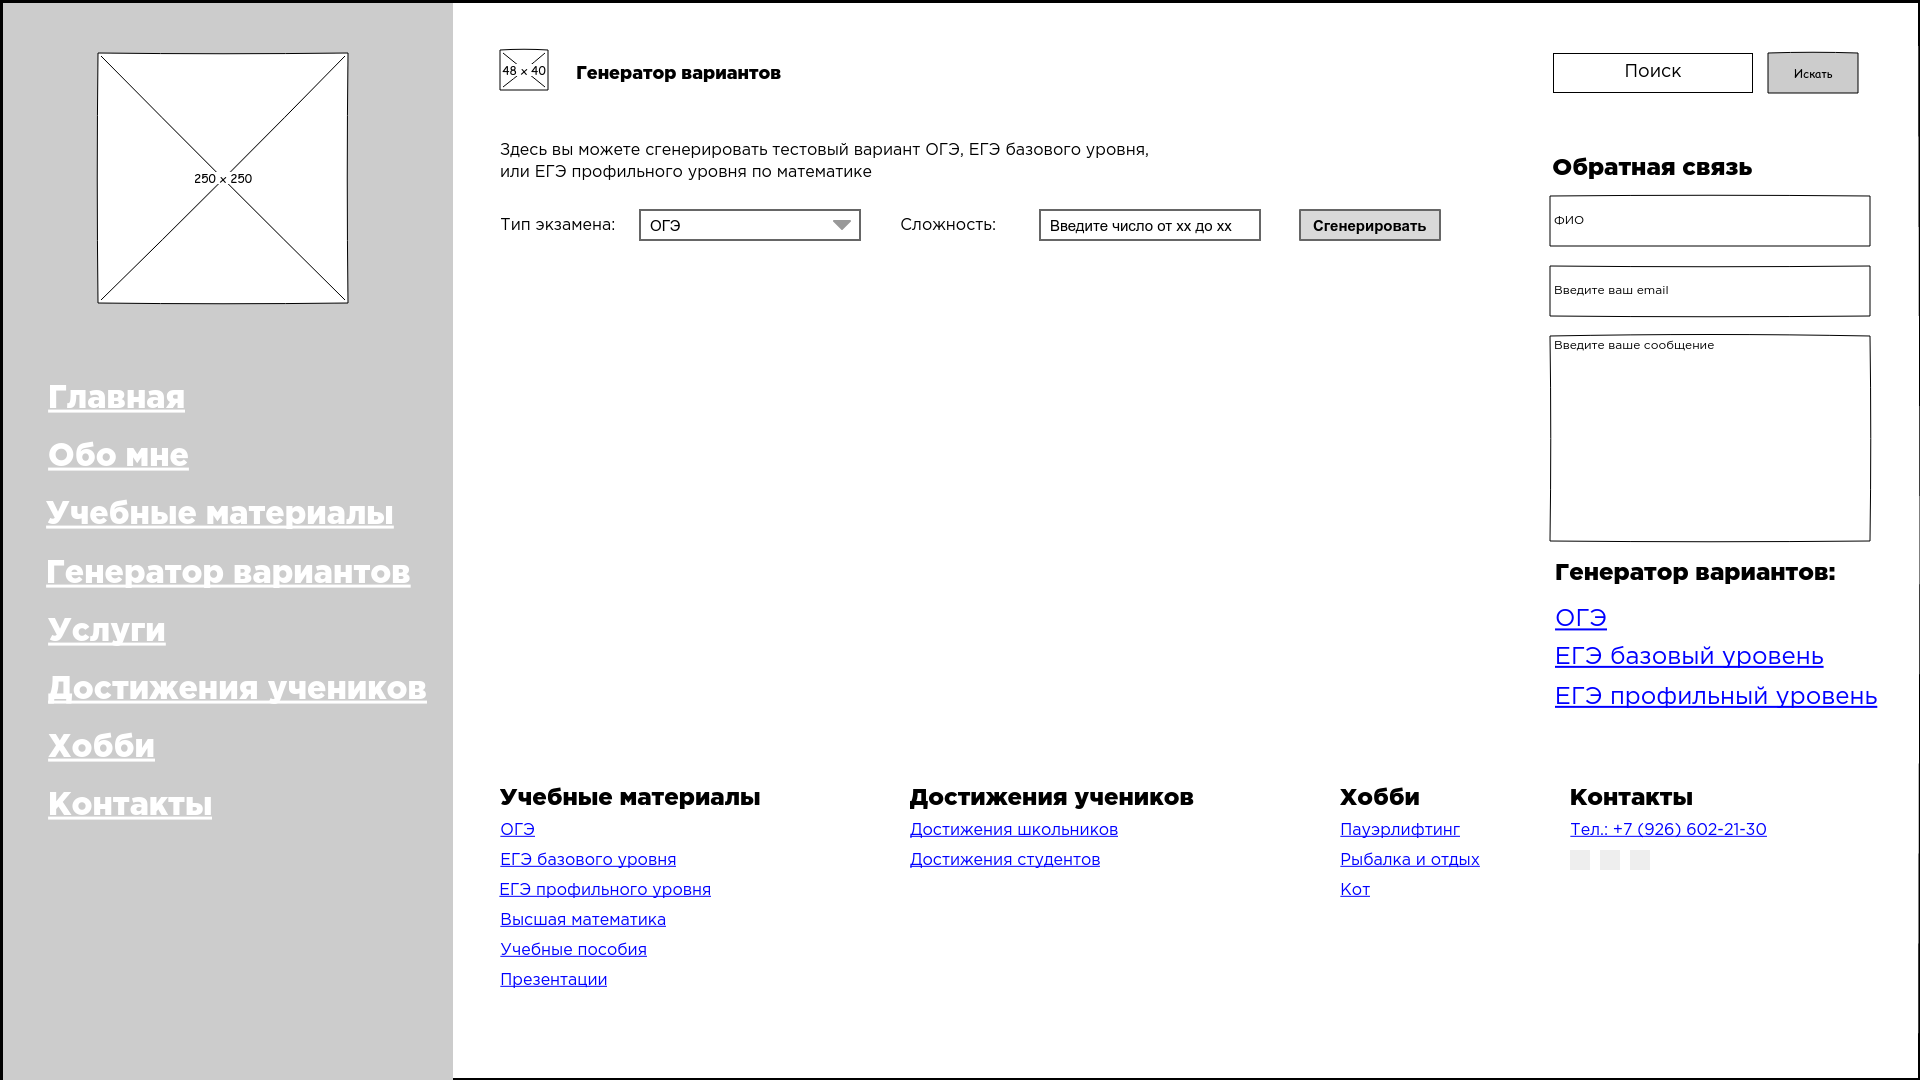
\includegraphics[width=\textwidth]{5-3-2}
\end{figure}
\paragraph{Назначение страницы:} Страница предназначена для генерации тестовых вариантов по математике из категорий «ЕГЭ профильный уровень», «ЕГЭ базовый уровень», «ОГЭ».

\paragraph{Структура страницы}
\begin{enumerate}
	\item Шапка
	\begin{enumerate}
		\item «Хлебные крошки»
		\item Поиск
	\end{enumerate}

	\item Меню
	\begin{enumerate}
		\item Логотип
		\item Навигация
	\end{enumerate}

	\item Сайдбар
	\begin{enumerate}
		\item Форма обратной связи
		\item Ссылки на социальные сети
		\item Генератор вариантов
	\end{enumerate}

	\item Контент
	\begin{enumerate}
		\item Форма генерации тестового варианта
		\begin{itemize}
			\item Поля выбора
			\begin{enumerate}
				\item Тип экзамена
				\item Сложность
			\end{enumerate}

			\item Кнопки управления
			\begin{enumerate}
				\item Сгенерировать
			\end{enumerate}
		\end{itemize}
	\end{enumerate}

	\item Футер
	\begin{enumerate}
		\item Навигация
	\end{enumerate}
\end{enumerate}

\paragraph{Функциональные возможности}
\begin{enumerate}
	\item Шапка
	\begin{enumerate}
		\item «Хлебные крошки»
		\begin{itemize}
			\item Навигация по разделам сайта
		\end{itemize}
		\item Поиск
		\begin{itemize}
			\item Поиск по сайту
		\end{itemize}
	\end{enumerate}

	\item Меню
	\begin{enumerate}
		\item Навигация
		\begin{itemize}
			\item Переход между разделами
		\end{itemize}
	\end{enumerate}

	\item Сайдбар
	\begin{enumerate}
		\item Форма обратной связи
		\begin{itemize}
			\item Отправка сообщений администрации сайта
		\end{itemize}

		\item Ссылки на социальные сети
		\begin{itemize}
			\item Переход на страницы социальных
		\end{itemize}

		\item Генератор вариантов
		\begin{itemize}
			\item Переход в раздел «Генератор вариантов»
		\end{itemize}
	\end{enumerate}

	\item Контент
	\begin{enumerate}
		\item Форма генерации тестового варианта
		\begin{itemize}
		\item Поля выбора
		\begin{enumerate}
			\item Выбор типа генерируемого экзамена
			\item Выбор сложности тестового варианта
		\end{enumerate}

		\item Кнопки управления
		\begin{enumerate}
			\item Генерация тестового варианта
		\end{enumerate}
		\end{itemize}
	\end{enumerate}

	\item Футер
	\begin{enumerate}
		\item Навигация
		\begin{itemize}
			\item Дополнительная навигация по сайту
		\end{itemize}
	\end{enumerate}
\end{enumerate}


\subsubsection{Страница «Задания»}
\begin{figure}[H]
	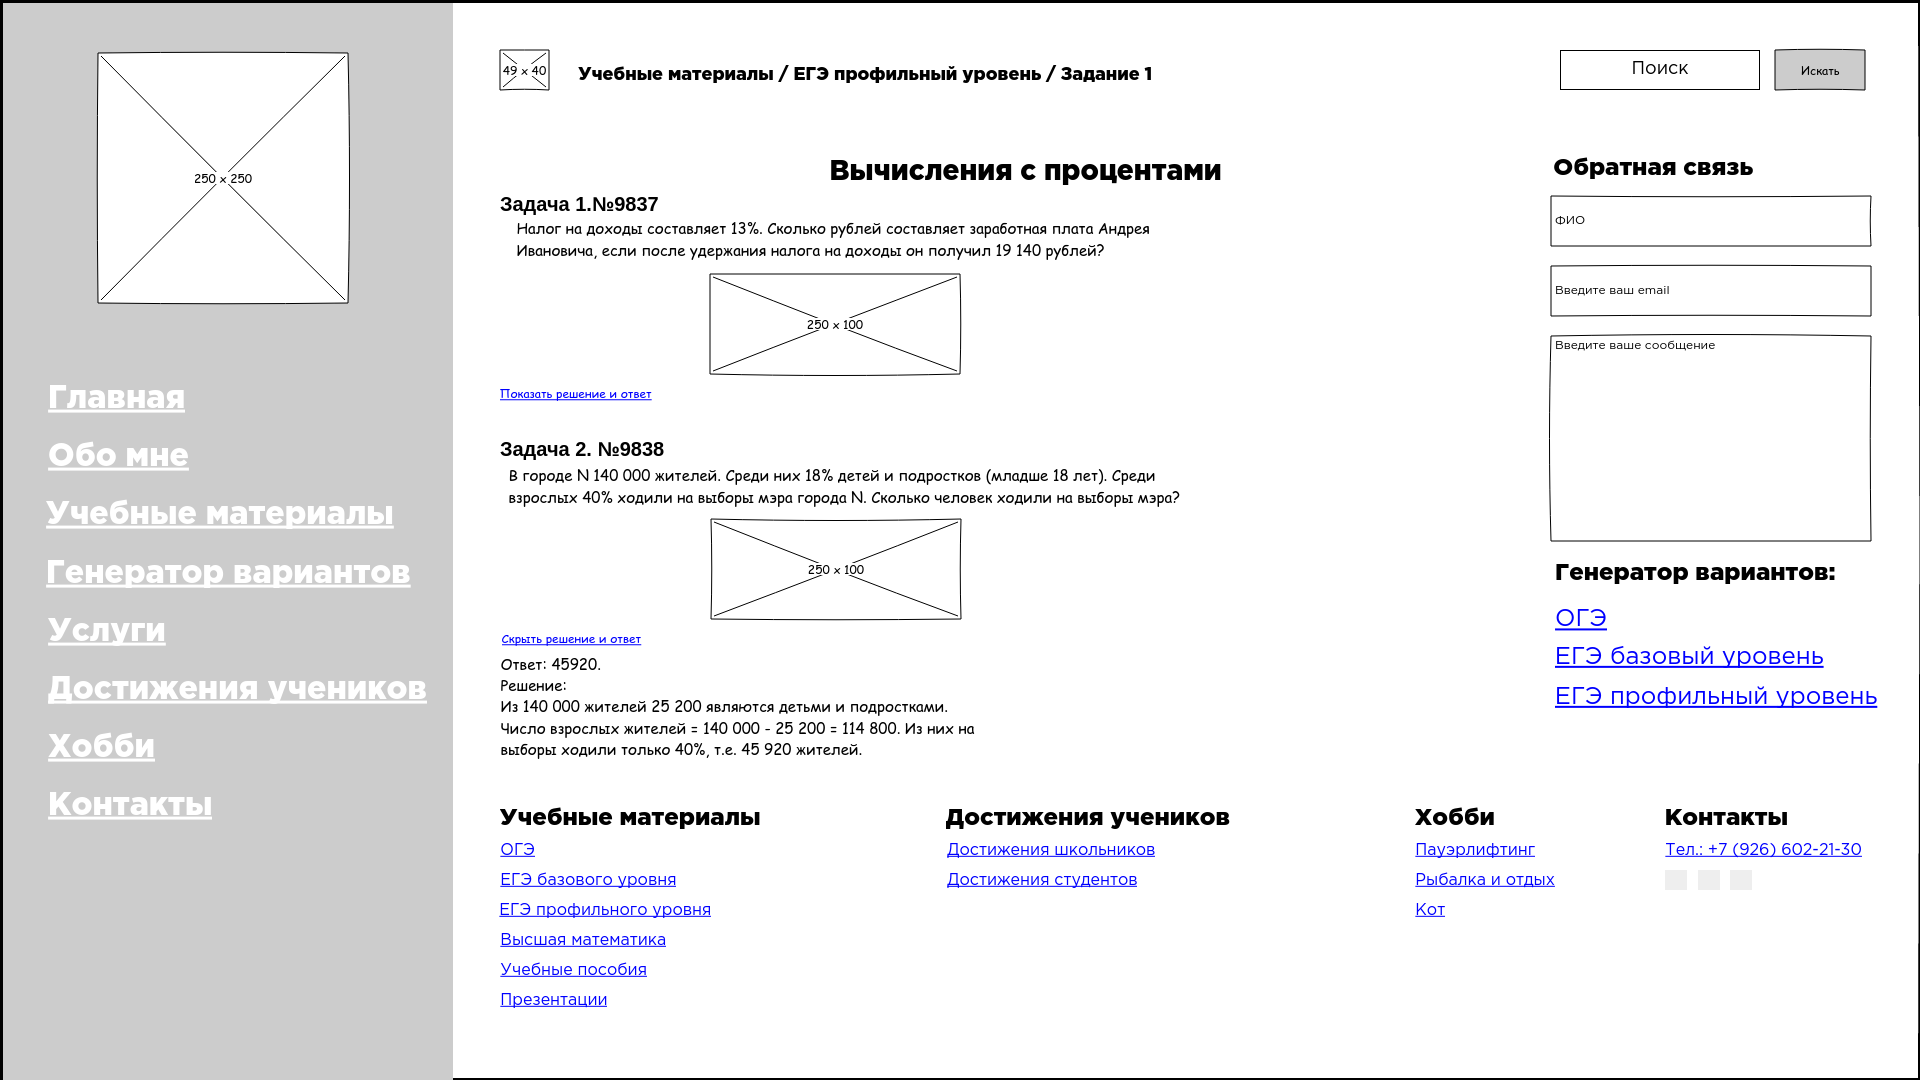
\includegraphics[width=\textwidth]{5-3-3}
\end{figure}
\paragraph{Назначение страницы:} Страница предназначена для публикации заданий по математике из категорий «ЕГЭ профильный уровень», «ЕГЭ базовый уровень», «ОГЭ».

\paragraph{Структура страницы}
\begin{enumerate}
	\item Шапка
	\begin{enumerate}
		\item «Хлебные крошки»
		\item Поиск
	\end{enumerate}

	\item Меню
	\begin{enumerate}
		\item Логотип
		\item Навигация
	\end{enumerate}

	\item Сайдбар
	\begin{enumerate}
		\item Форма обратной связи
		\item Ссылки на социальные сети
		\item Генератор вариантов
	\end{enumerate}

	\item Контент
	\begin{enumerate}
		\item Список задач
		\begin{itemize}
		\item Заголовок списка
		\item Задача
		\begin{enumerate}
			\item Заголовок задачи
			\item Условие
			\item Решение и ответ
		\end{enumerate}
		\end{itemize}
	\end{enumerate}

	\item Футер
	\begin{enumerate}
		\item Навигация
	\end{enumerate}
\end{enumerate}

\paragraph{Функциональные возможности}
\begin{enumerate}
	\item Шапка
	\begin{enumerate}
		\item «Хлебные крошки»
		\begin{itemize}
			\item Навигация по разделам сайта
		\end{itemize}
		\item Поиск
		\begin{itemize}
			\item Поиск по сайту
		\end{itemize}
	\end{enumerate}

	\item Меню
	\begin{enumerate}
		\item Навигация
		\begin{itemize}
			\item Переход между разделами
		\end{itemize}
	\end{enumerate}

	\item Сайдбар
	\begin{enumerate}
		\item Форма обратной связи
		\begin{itemize}
			\item Отправка сообщений администрации сайта
		\end{itemize}

		\item Ссылки на социальные сети
		\begin{itemize}
			\item Переход на страницы социальных
		\end{itemize}

		\item Генератор вариантов
		\begin{itemize}
			\item Переход в раздел «Генератор вариантов»
		\end{itemize}
	\end{enumerate}

	\item Контент
	\begin{enumerate}
		\item Список задач
		\begin{itemize}
		\item Задача
		\begin{enumerate}
			\item Просмотр условий, решений и ответов задач
		\end{enumerate}
		\end{itemize}
	\end{enumerate}

	\item Футер
	\begin{enumerate}
		\item Навигация
		\begin{itemize}
			\item Дополнительная навигация по сайту
		\end{itemize}
	\end{enumerate}
\end{enumerate}


\subsubsection{Страница «Авторизация»}
\begin{figure}[H]
	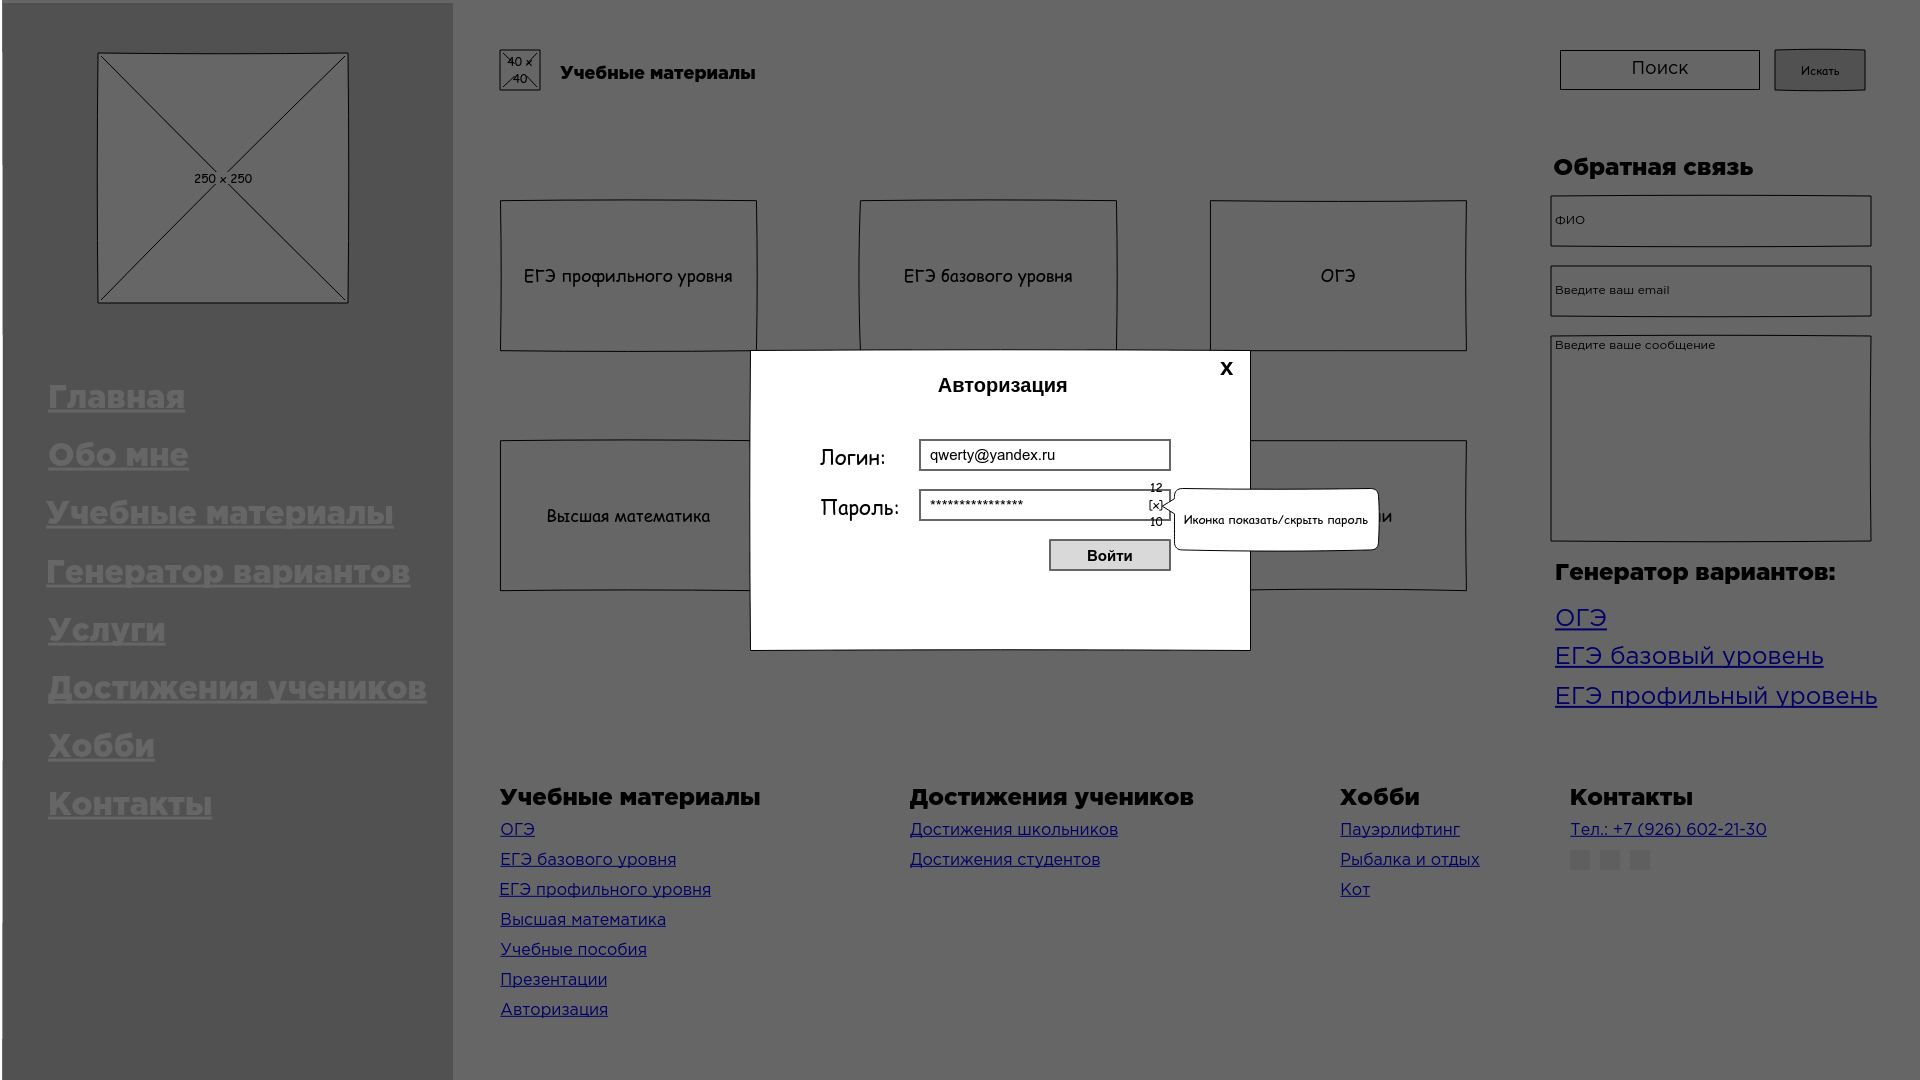
\includegraphics[width=\textwidth]{5-3-4}
\end{figure}
\paragraph{Назначение страницы:} Страница предназначена для входа в панель управления разделами «Учебные материалы» и «Генератор вариантов».

\paragraph{Структура страницы}
\begin{enumerate}
	\item Окно авторизации
	\begin{enumerate}
		\item Поля авторизации
		\begin{itemize}
		\item Логин
		\item Пароль
		\end{itemize}
		\item Кнопки управления
		\begin{itemize}
		\item Войти
		\end{itemize}
	\end{enumerate}
\end{enumerate}

\paragraph{Функциональные возможности}
\begin{enumerate}
	\item Окно авторизации
	\begin{enumerate}
		\item Вход в административную панель
	\end{enumerate}
\end{enumerate}


\subsubsection{Страница «Сгенерированный вариант»}
\begin{figure}[H]
	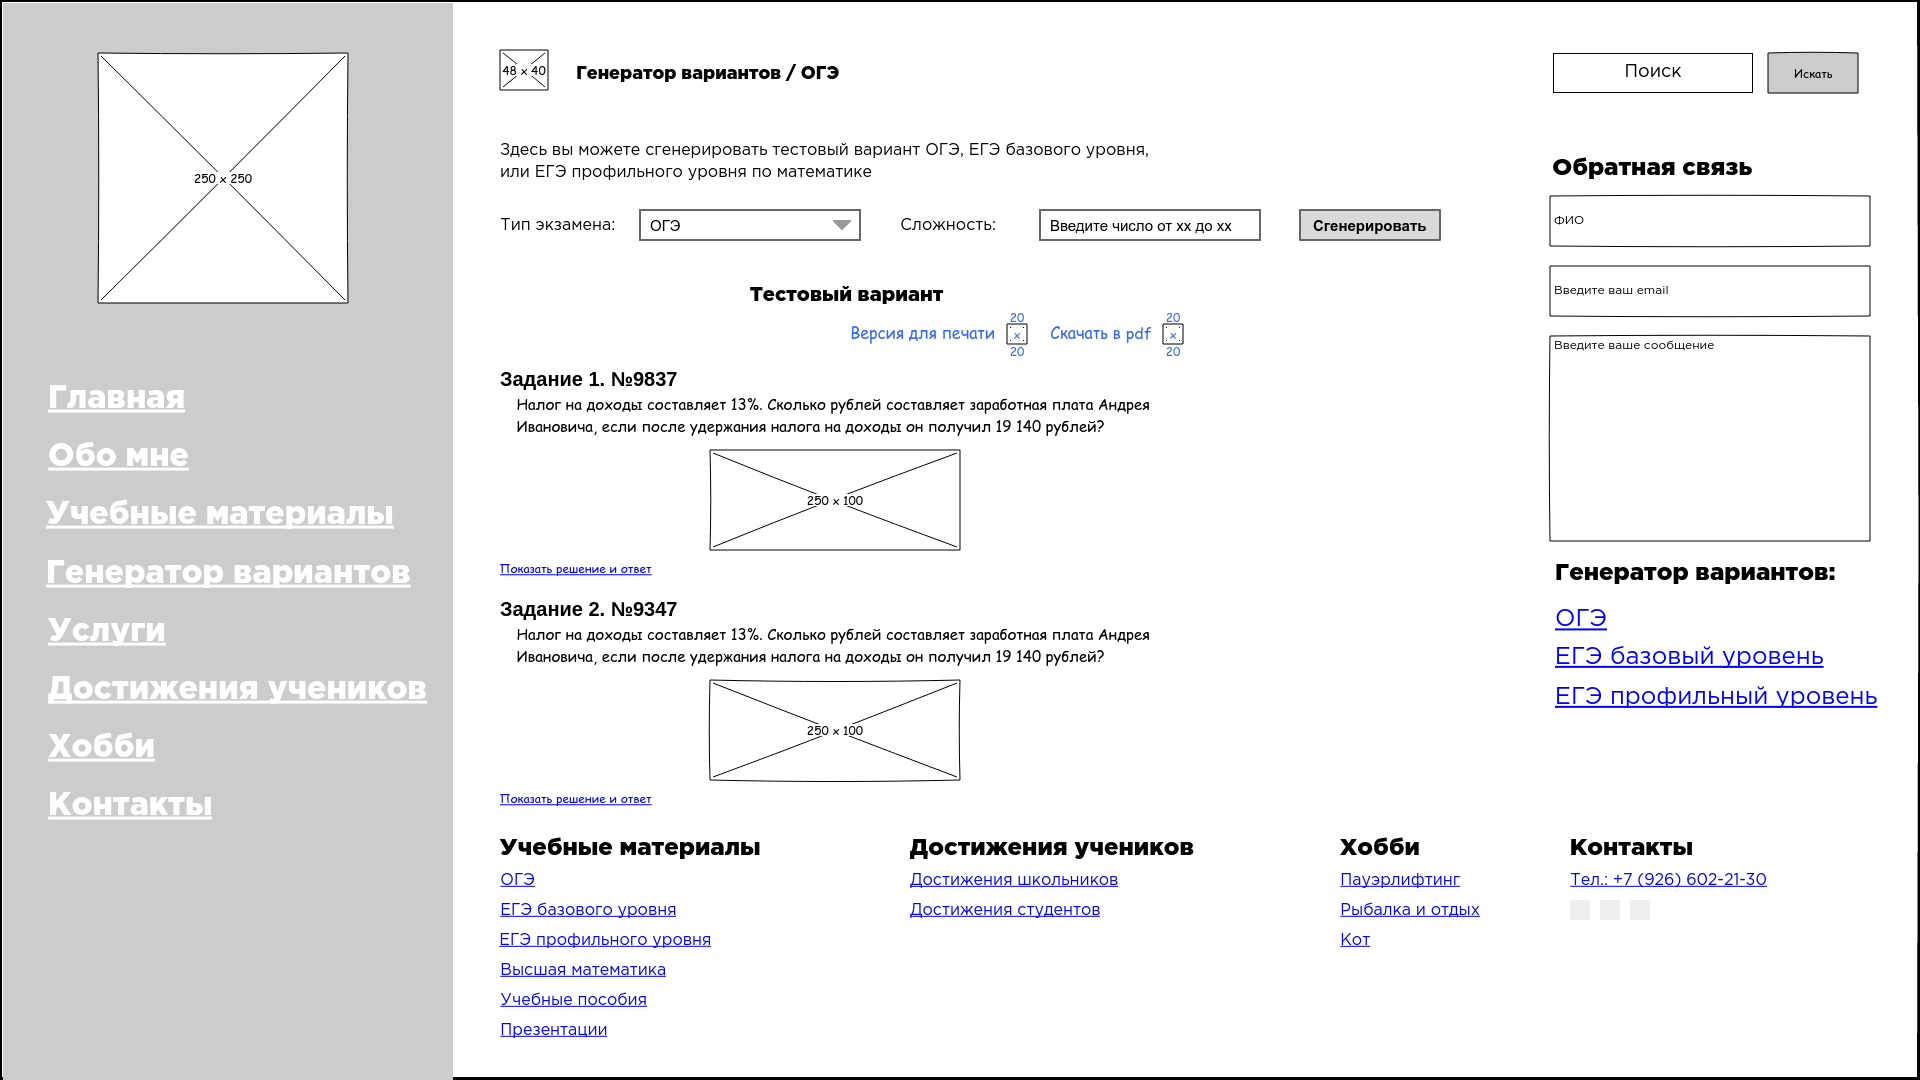
\includegraphics[width=\textwidth]{5-3-5}
\end{figure}
\paragraph{Назначение страницы:} Страница предназначена для решения тестового варианта по математике из категорий «ЕГЭ профильный уровень», «ЕГЭ базовый уровень», «ОГЭ».

\paragraph{Структура страницы}
\begin{enumerate}
	\item Шапка
	\begin{enumerate}
		\item «Хлебные крошки»
		\item Поиск
	\end{enumerate}

	\item Меню
	\begin{enumerate}
		\item Логотип
		\item Навигация
	\end{enumerate}

	\item Сайдбар
	\begin{enumerate}
		\item Форма обратной связи
		\item Ссылки на социальные сети
		\item Генератор вариантов
	\end{enumerate}

	\item Контент
	\begin{enumerate}
		\item Форма генерации тестового варианта
		\begin{itemize}
		\item Поля выбора
		\item Кнопки управления
		\end{itemize}

		\item Тестовый вариант
		\begin{itemize}
		\item Ссылки на версии для скачивания и печати
		\item Заголовок списка
		\item Задачи
		\begin{enumerate}
			\item Заголовок задачи
			\item Условие
			\item Решение и ответ
		\end{enumerate}
		\end{itemize}
	\end{enumerate}

	\item Футер
	\begin{enumerate}
		\item Навигация
	\end{enumerate}
\end{enumerate}

\paragraph{Функциональные возможности}
\begin{enumerate}
	\item Шапка
	\begin{enumerate}
		\item «Хлебные крошки»
		\begin{itemize}
			\item Навигация по разделам сайта
		\end{itemize}
		\item Поиск
		\begin{itemize}
			\item Поиск по сайту
		\end{itemize}
	\end{enumerate}

	\item Меню
	\begin{enumerate}
		\item Навигация
		\begin{itemize}
			\item Переход между разделами
		\end{itemize}
	\end{enumerate}

	\item Сайдбар
	\begin{enumerate}
		\item Форма обратной связи
		\begin{itemize}
			\item Отправка сообщений администрации сайта
		\end{itemize}

		\item Ссылки на социальные сети
		\begin{itemize}
			\item Переход на страницы социальных
		\end{itemize}

		\item Генератор вариантов
		\begin{itemize}
			\item Переход в раздел «Генератор вариантов»
		\end{itemize}
	\end{enumerate}

	\item Контент
	\begin{enumerate}
		\item Форма генерации тестового варианта
		\begin{itemize}
		\item Поля выбора
		\begin{enumerate}
			\item Выбор типа генерируемого экзамена
			\item Выбор сложности тестового варианта
		\end{enumerate}
		\item Кнопки управления
		\begin{enumerate}
			\item Генерация тестового варианта
		\end{enumerate}
		\end{itemize}

		\item Тестовый вариант
		\begin{itemize}
		\item Ссылки на версии для скачивания и печати
		\begin{enumerate}
			\item Открытие версии для скачивания,или версии для печати
		\end{enumerate}
		\item Задачи
		\begin{enumerate}
			\item Просмотр условий, решений и ответов задач
		\end{enumerate}
		\end{itemize}
	\end{enumerate}

	\item Футер
	\begin{enumerate}
		\item Навигация
		\begin{itemize}
			\item Дополнительная навигация по сайту
		\end{itemize}
	\end{enumerate}
\end{enumerate}


\subsubsection{Страница «Версия для печати»}

Прототип страницы прилагается к данному техническому заданию в виде png-файла.

\paragraph{Назначение страницы:} Страница предназначена для печати тестового варианта по математике из категорий «ЕГЭ профильный уровень», «ЕГЭ базовый уровень», «ОГЭ».

\paragraph{Структура страницы}
\begin{enumerate}
	\item Тестовый вариант
	\begin{enumerate}
		\item Заголовок
		\item Подзаголовок
		\item Список задач
		\begin{itemize}
		\item Задача
		\begin{enumerate}
			\item Просмотр условий, решений и ответов задач
		\end{enumerate}
		\end{itemize}
		\item Таблица с ответами
	\end{enumerate}
\end{enumerate}

\paragraph{Функциональные возможности:} Печать тестового варианта.


\subsubsection{Страница «Версия для скачивания»}

Прототип страницы прилагается к данному техническому заданию в виде png-файла.

\paragraph{Назначение страницы:} Страница предназначена для скачивания тестового варианта по математике из категорий «ЕГЭ профильный уровень», «ЕГЭ базовый уровень», «ОГЭ».

\paragraph{Структура страницы}
\begin{enumerate}
	\item Тестовый вариант
	\begin{enumerate}
		\item Заголовок
		\item Подзаголовок
		\item Список задач
		\begin{itemize}
		\item Задача
		\begin{enumerate}
			\item Просмотр условий, решений и ответов задач
		\end{enumerate}
		\end{itemize}
		\item Таблица с ответами
		\item Список решений с ответами
	\end{enumerate}
\end{enumerate}

\paragraph{Функциональные возможности:} Скачивание тестового варианта в формате pdf.
